% RESULTADOS Y DISCUSION 

\cleardoublepage

\chapter{Experimentación}
\label{experimentacion}

\section{Introducción}
\label{resultados-introduccion}

A continuación haremos un repaso de los resultados obtenidos en el subconjunto de experimentos más representativo, realizados con los diferentes algoritmos propuestos.
\medskip

Detallaremos brevemente también las conclusiones parciales que obtenemos en cada experimento, así como posibles soluciones a los problemas que se nos plantean en cada uno.
\medskip

Debido al coste computacional de ejecutar cada experimento sobre el conjunto de datos total, cada experimento se compone de subexperimentos previos, en los cuales intentábamos probar nuestras soluciones con un conjunto de datos menor al original, alrededor de unas 20 imágenes. 
\medskip

La idea detrás de esta subexperimentación era conseguir un modelo de agente que sea capaz de realizar \textit{overfitting} sobre el conjunto de datos de manera relativamente rápida y que obtuviese una convergencia tanto en la recompensa obtenida tanto en las imágenes del conjunto de entrenamiento como en el conjunto de test como en el número de pasos que realizaba sobre cada una de las imágenes. Esto nos permitió también acortar el tiempo entre las diferentes pruebas, ya que el conseguir este overfitting nos aseguraba que el agente seguiría en un principio las ideas que queríamos implementar y además provocó que pudiesemos experimentar con diferentes definiciones tanto de nuestra recompensa como de nuestro entorno, así como hacer \textit{fine tunning} de nuestros hiperparámetros.
\medskip

Ligado a la subexperimentación comentada, en cuanto a los hiperparámetros, vimos como el learning rate jugaba un papel muy importante en todos y cada uno de los algoritmos usados. Un \textit{learning rate} muy alto hacía que nuestros agentes solo tomasen una decisión, llevando a escorarse practicamente hacia un lado en todas las ocasiones. Por otro lado, un \textit{learning rate} muy bajo no permitía que nuestro agente fuese capaz muchas veces de tomar una decisión clara, y aunque esto pueda entenderse como parte de la exploración del agente muchas veces no permitía al agente obtener la recompensa máxima del entorno en el número máximo de pasos que se había establecido y obtenía por lo tanto solo recompensas parciales.
\medskip

Durante los experimentos podremos comprobar que en alguno de ellos el número de métricas que mostraremos es más alto que en otros, esto no es solo debido a que queramos destacar una cualidad específica del experimento, sino que tambien formó parte de la experimentación y el descubrimiento de algunos de los problemas que nos fuimos encontrando, que nos llevó a tener que realizar el seguimiento de algunos aspectos del entrenamiento que no estaban contemplados en experimentos anteriores. Estos problemas estuvieron relacionados principalmente con la convergencia en la toma de decisiones del agente tal y como se discutirá más adelante.
\medskip

Por último también mostraremos algunos resultados de las imágenes que fuimos obteniendo en cada caso. Cabe recordar que la ejecución del agente durante el test se detiene cuando decide ejecutar la acción de permanecer quieto, y que tanto esta recompensa como el número de acciones hasta llegar a ella se tienen en cuenta como medidas subjetivas de la eficacia del agente, tal y como comentamos en la sección \ref{evaluacion}.
\medskip

El total de los experimentos está disponible en el repositorio de \href{https://github.com/lucaswerner90/msc-degree-ai}{GitHub} para un análisis más extenso y se adjunta el título de cada uno de ellos en el Apéndize \ref{apendize-a}. 
\medskip

La herramienta utilizada para monitorear el progreso de las diferentes métricas durante los diferentes entrenamientos es \href{https://www.tensorflow.org/tensorboard?hl=es-419}{Tensorboard}, ya que además de su facil integración con \href{https://pytorch.org/}{PyTorch} nos permitía comparar dichas métricas entre los diferentes experimentos.
\medskip

\section{Policy Gradient}
\label{resultados-policy-gradient}

El algoritmo \textit{Policy Gradient} fue nuestra primera opción a la hora de implementar nuestro agente. Se buscaba obtener una primera aproximación a nuestro problema y buscábamos sobre todo tener un modelo que sirviese como \textit{baseline}, así como definir la estructura general de nuestro programa.
\medskip

\subsection{Experimento 1}
\label{resultados-policy-gradient-experimento-1}

En este primer experimento utilizamos como criterio de finalización del episodio que el agente realizase un máximo de 50 acciones o que obtuviese la máxima recompensa del entorno, en este caso se mantuvo la recompensa proporcional con la distancia al punto objetivo y no se hizo ninguna recompensa extra por llegar al final del episodio correctamente.
\medskip

\begin{figure}[H]
	\centering
	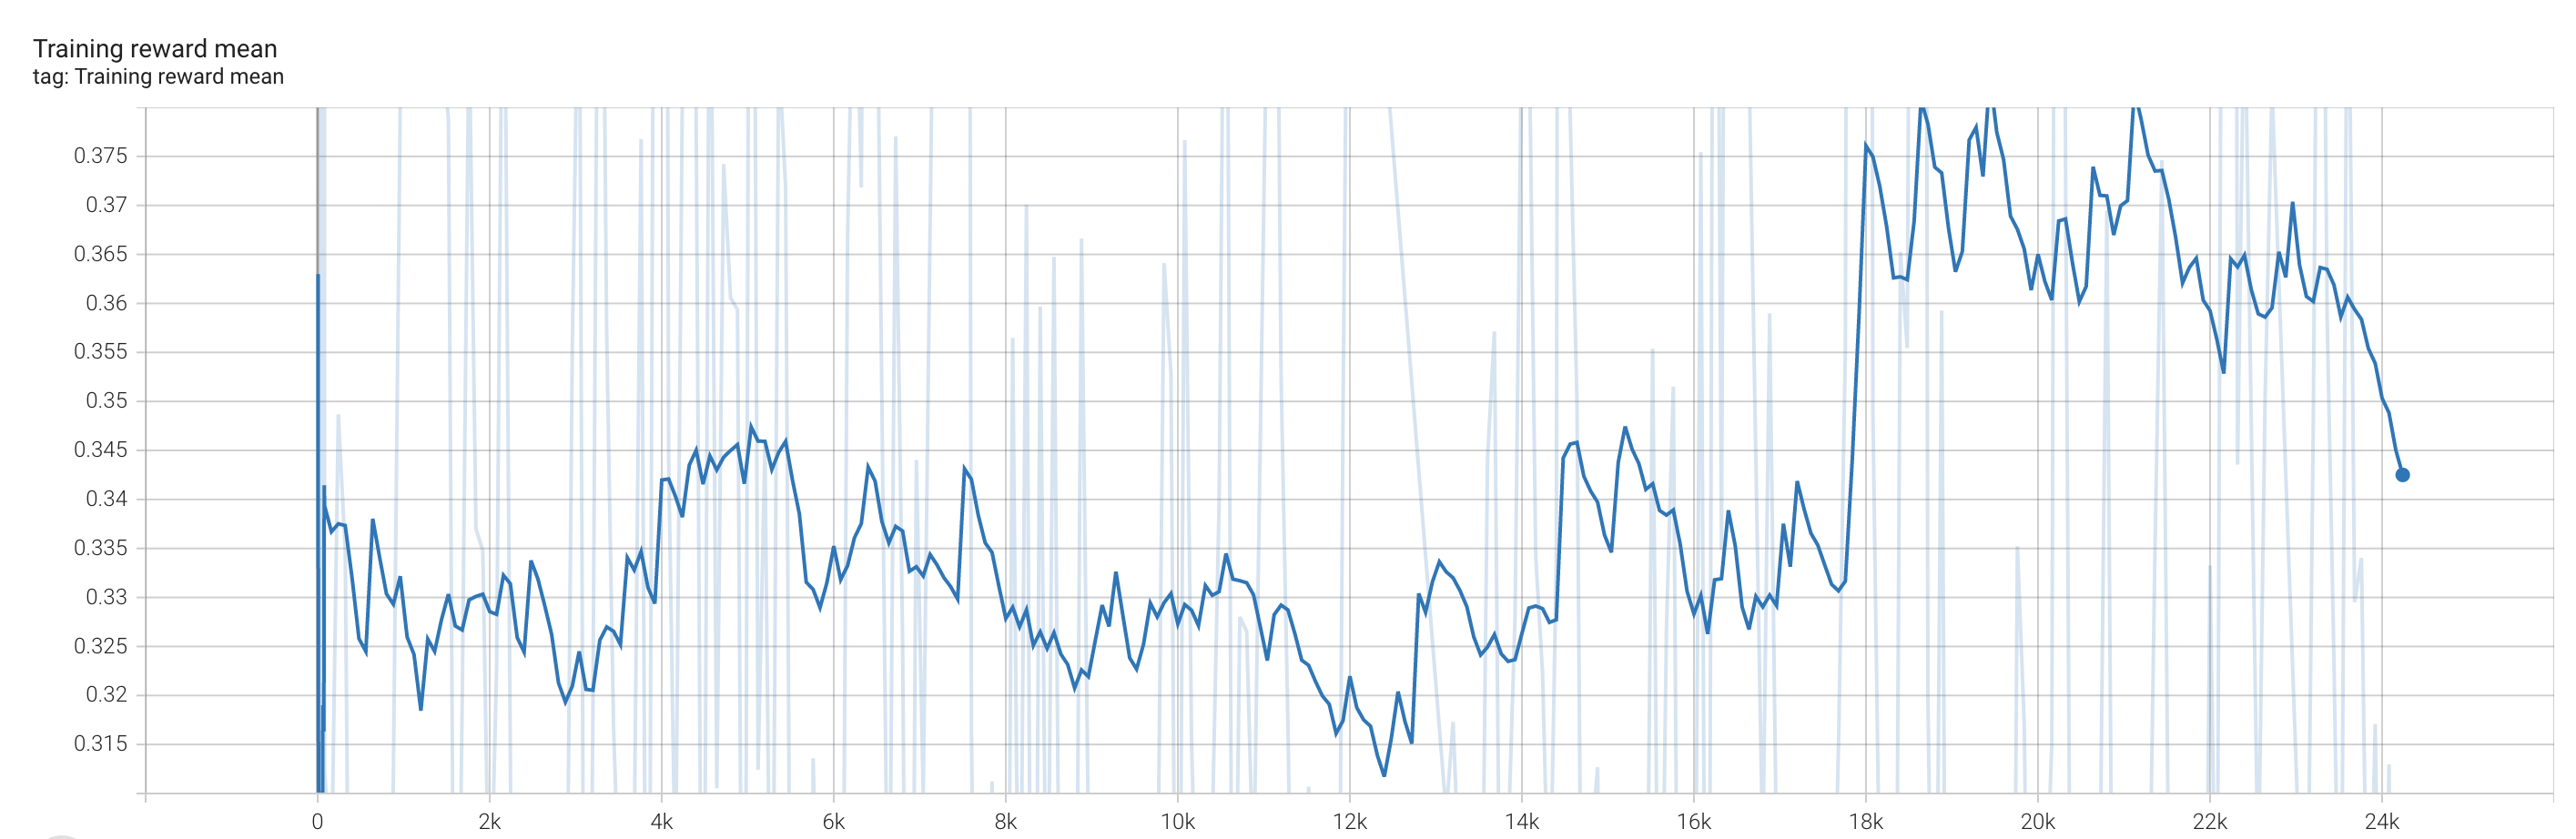
\includegraphics[width=1\textwidth]{figuras/experiments/policy_gradient/policy_gradient_normalized_image_reward_20_epochs/training_reward_mean.png}
	\caption[Experimento Policy Gradient 1 - Recompensa media en el conjunto de entrenamiento]{Experimento Policy Gradient 1 - Recompensa media en el conjunto de entrenamiento}
	\label{fig-experimento-policy-gradient-1-training-reward-mean}
\end{figure}

\begin{figure}[H]
	\centering
	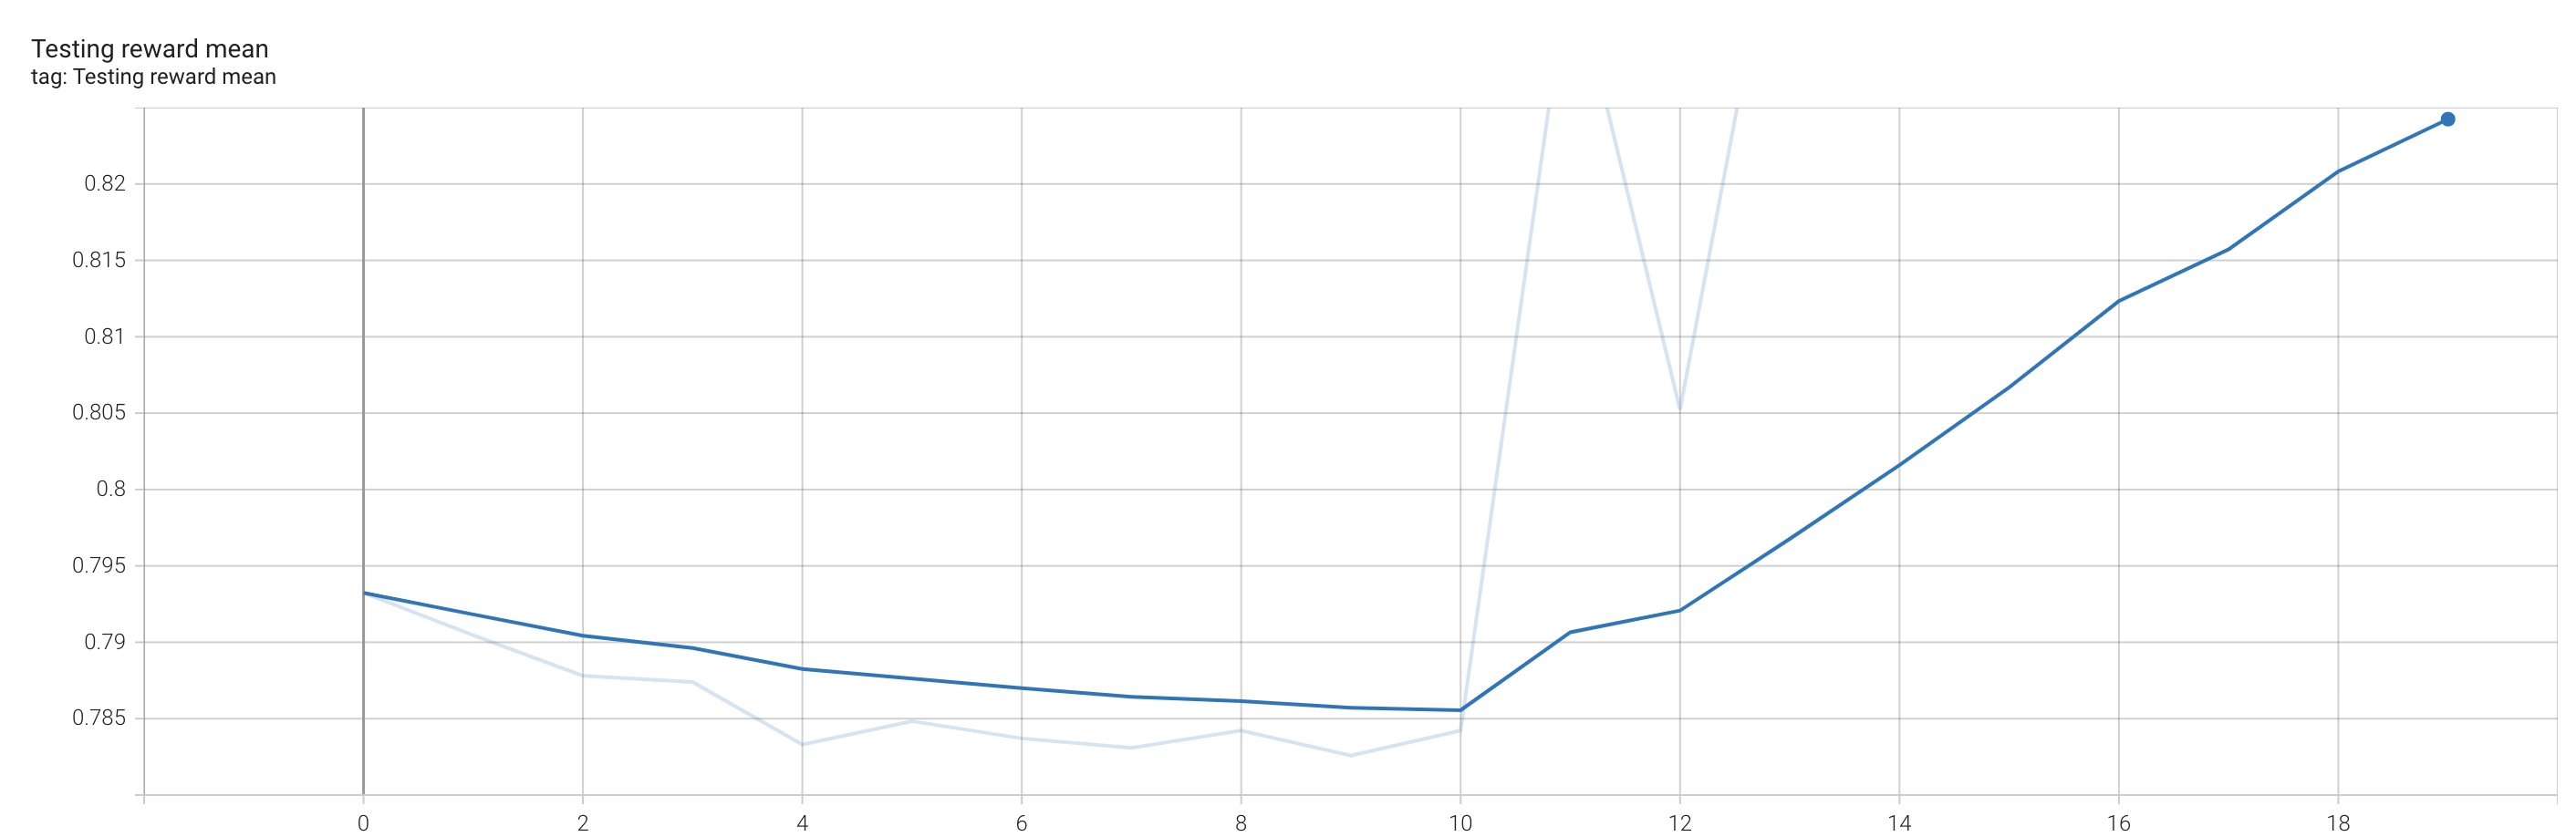
\includegraphics[width=1\textwidth]{figuras/experiments/policy_gradient/policy_gradient_normalized_image_reward_20_epochs/testing_reward_mean.png}
	\caption[Experimento Policy Gradient 1 - Testing reward mean]{Experimento Policy Gradient 1 - Testing reward mean}
	\label{fig-experimento-policy-gradient-1-testing-reward-mean}
\end{figure}
\begin{figure}[H]
	\centering
	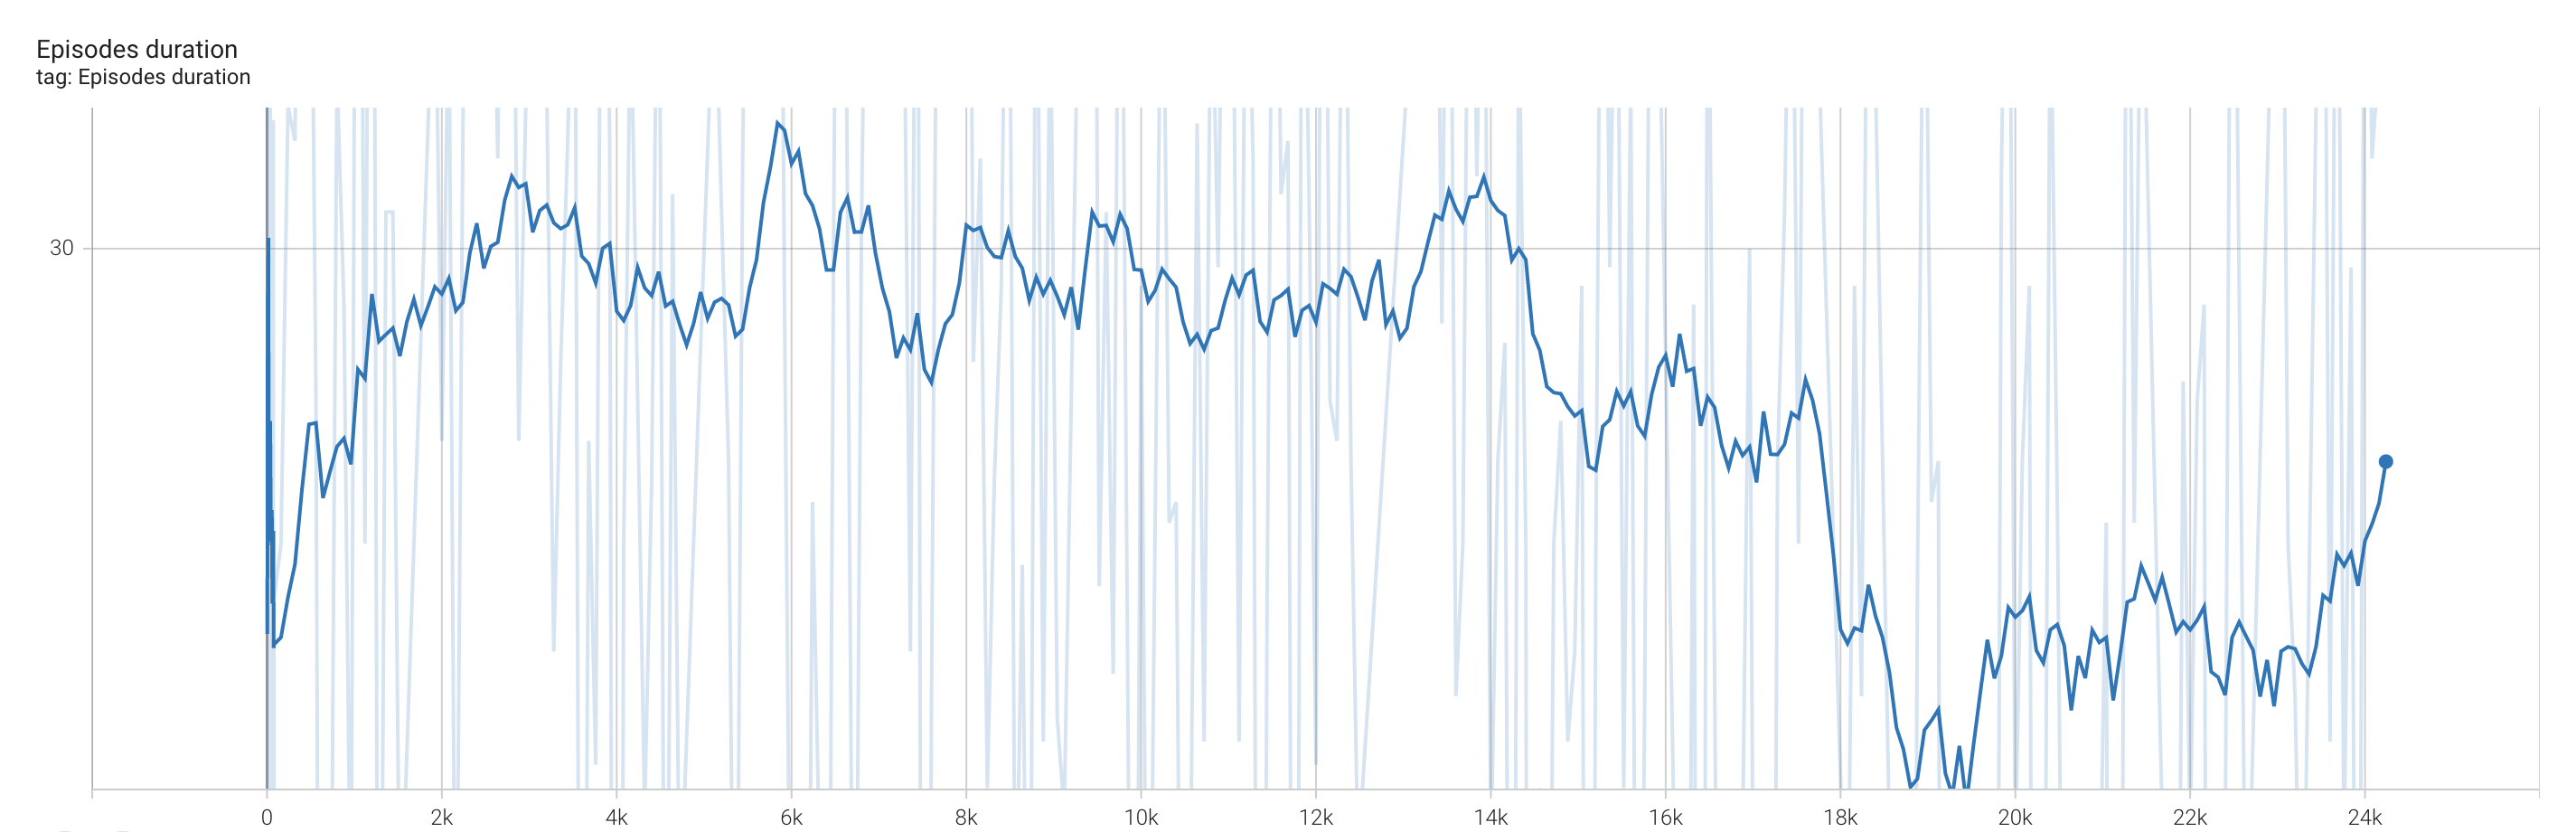
\includegraphics[width=1\textwidth]{figuras/experiments/policy_gradient/policy_gradient_normalized_image_reward_20_epochs/episodes_duration.png}
	\caption[Experimento Policy Gradient 1 - Duración de los episodios]{Experimento Policy Gradient 1 - Duración de los episodios}
	\label{fig-experimento-policy-gradient-1-episodes-duration}
\end{figure}

Lo que se puede apreciar es que existe una tendencia a la baja de nuestro algoritmo en cuanto al número de acciones en el conjunto de entrenamiento. Por otra parte, se aprecia que la recompensa en el conjunto de test comienza a subir a partir de la época 10, lo cual marca un punto importante de inflexión en esta. 

\subsection{Experimento 2}
\label{resultados-policy-gradient-experimento-2}

Los parámetros utilizados en este experimento son similares al anterior, pero en este caso el entrenamiento se ejecuta durante unas 50 épocas, unas 30 más que el experimento \ref{resultados-policy-gradient-experimento-1}.
\medskip

\begin{figure}[H]
	\centering
	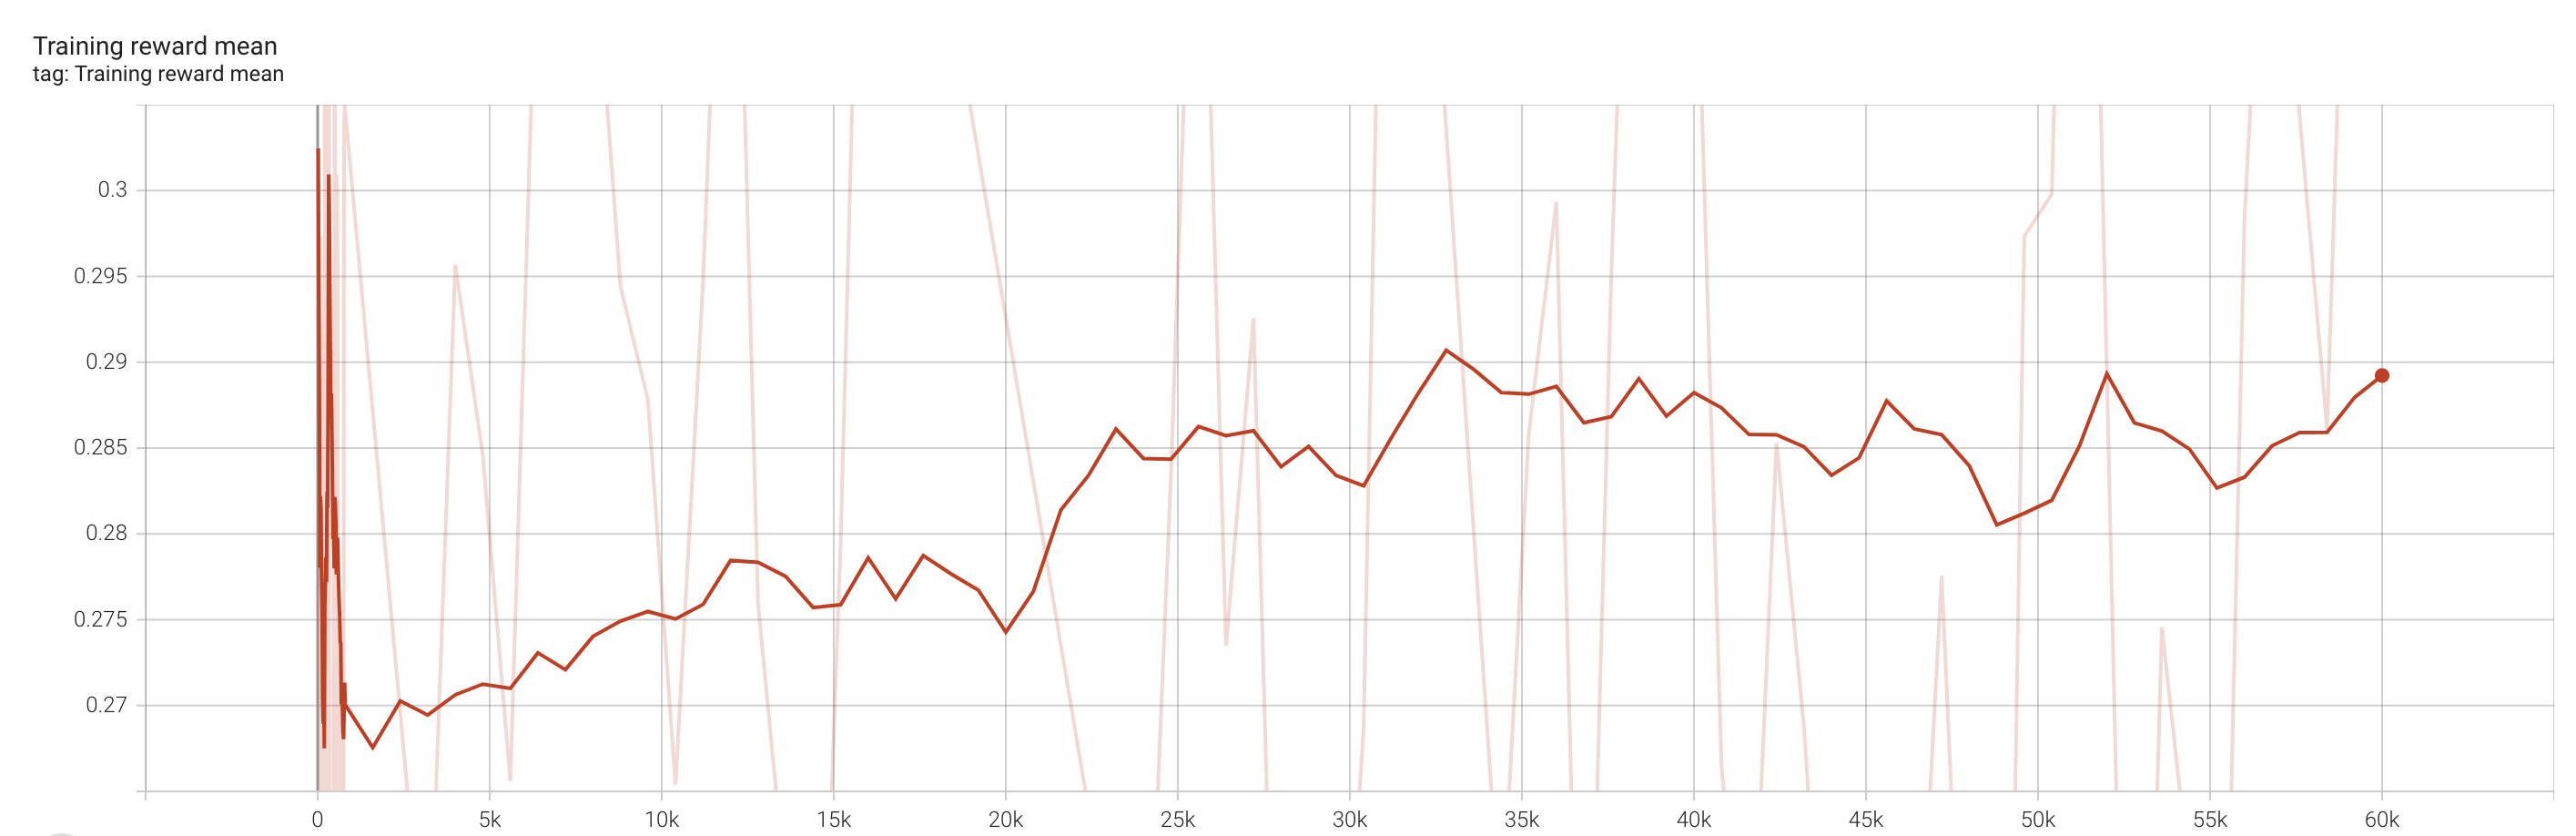
\includegraphics[width=1\textwidth]{figuras/experiments/policy_gradient/policy_gradient_normalized_image_reward_50_epochs/training_reward_mean.png}
	\caption[Experimento Policy Gradient 2 - Recompensa media en el conjunto de entrenamiento]{Experimento Policy Gradient 2 - Recompensa media en el conjunto de entrenamiento}
	\label{fig-experimento-policy-gradient-2-training-reward-mean}
\end{figure}
\begin{figure}[H]
	\centering
	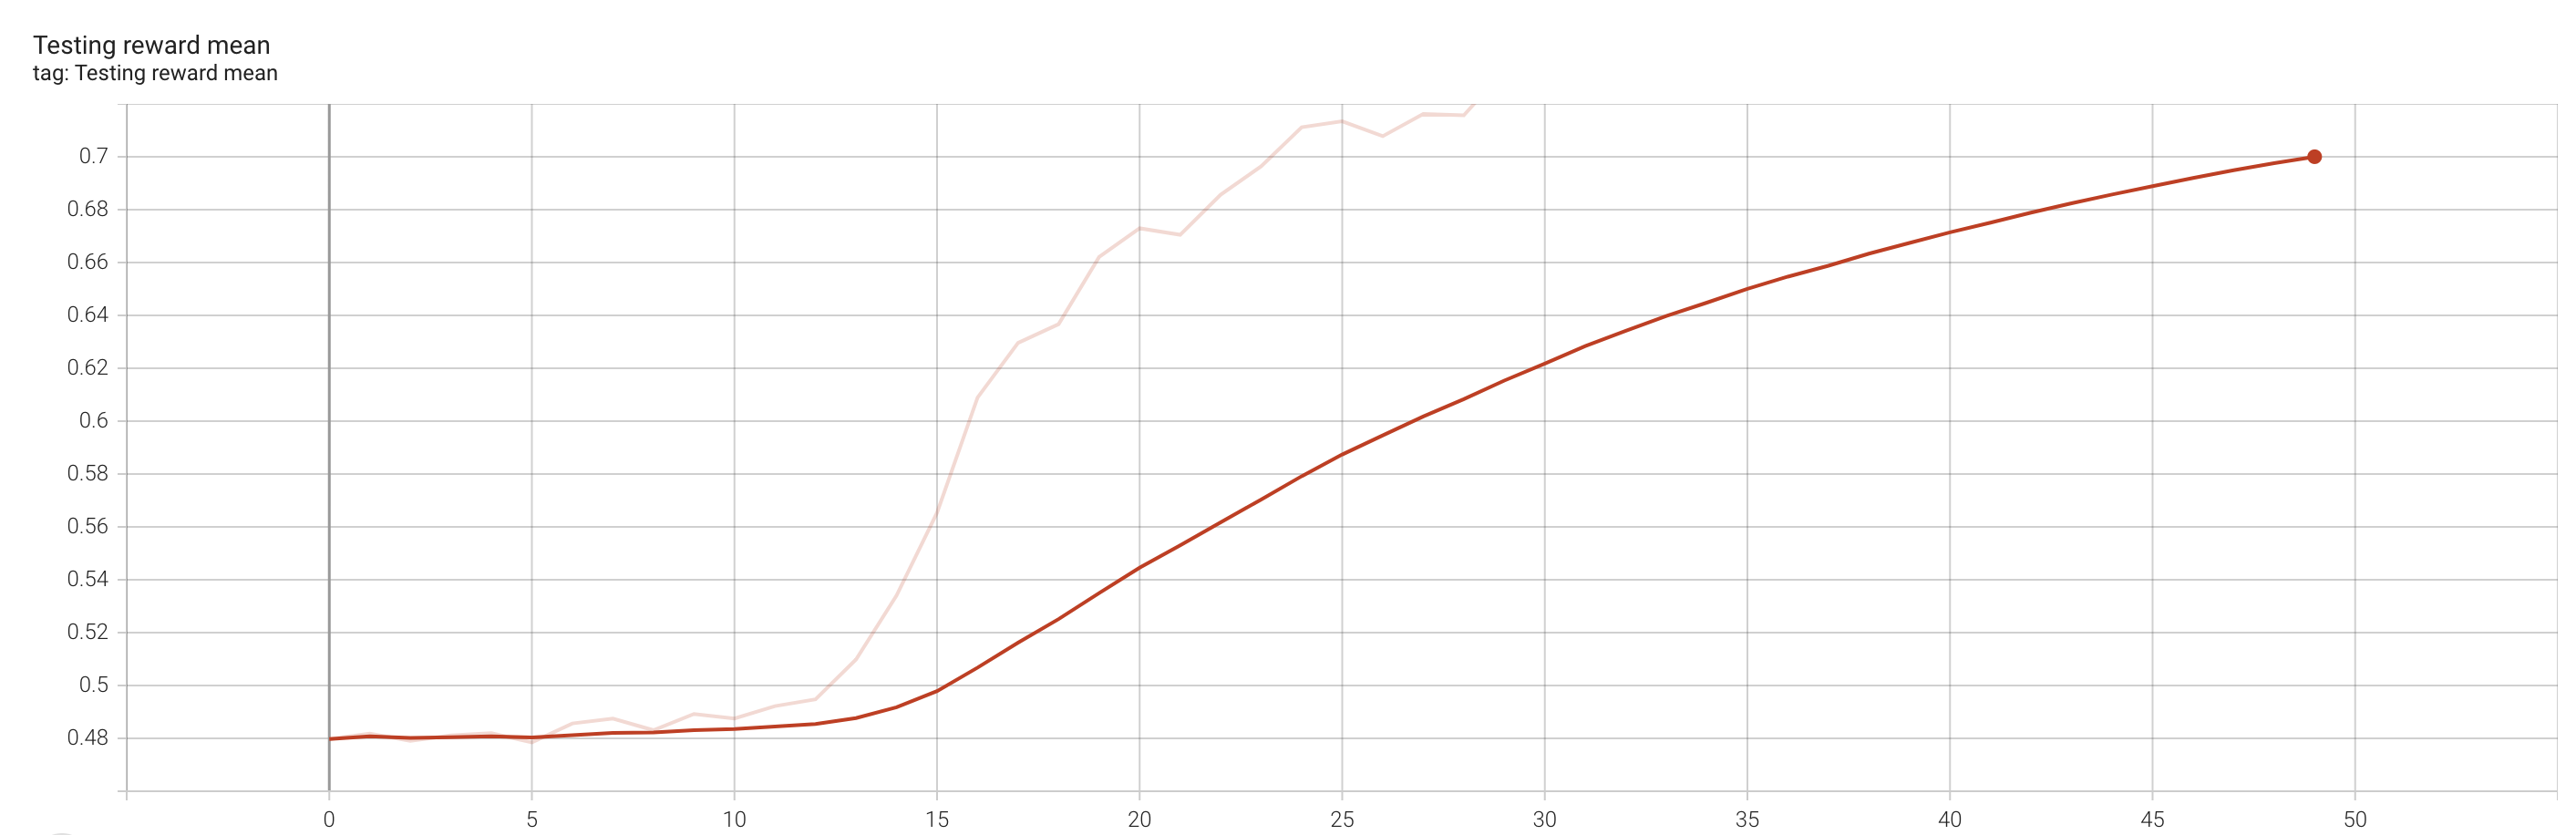
\includegraphics[width=1\textwidth]{figuras/experiments/policy_gradient/policy_gradient_normalized_image_reward_50_epochs/testing_reward_mean.png}
	\caption[Experimento Policy Gradient 2 - Testing reward mean]{Experimento Policy Gradient 2 - Testing reward mean}
	\label{fig-experimento-policy-gradient-2-testing-reward-mean}
\end{figure}
\begin{figure}[H]
	\centering
	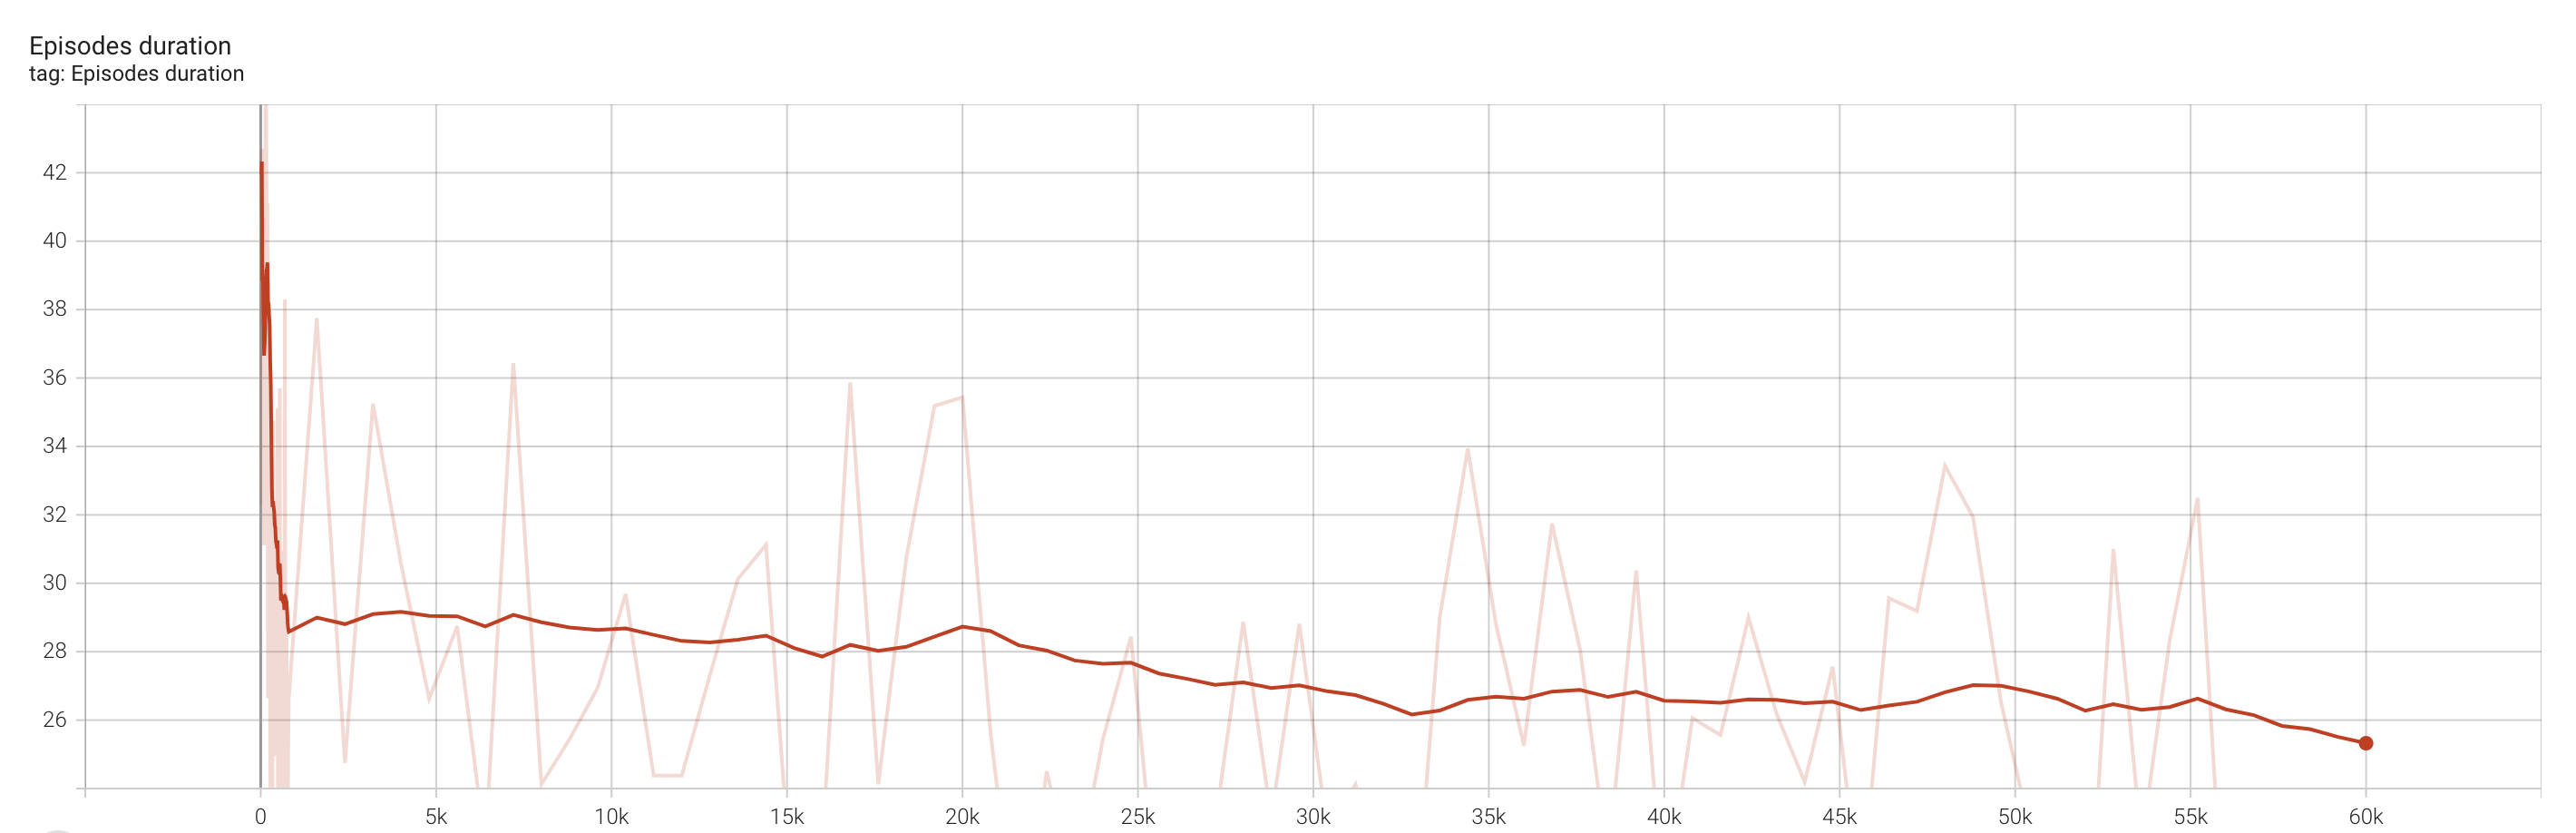
\includegraphics[width=1\textwidth]{figuras/experiments/policy_gradient/policy_gradient_normalized_image_reward_50_epochs/episodes_duration.png}
	\caption[Experimento Policy Gradient 2 - Duración de los episodios]{Experimento Policy Gradient 2 - Duración de los episodios}
	\label{fig-experimento-policy-gradient-2-episodes-duration}
\end{figure}

Vemos que en este experimento la tendencia que vimos en el experimento anterior se confirma: el número de acciones por imagen en el conjunto de entrenamiento parece seguir una tendencia a la baja y tanto la recompensa en el conjunto de test como en el entrenamiento aumentan según van avanzando las épocas.
\medskip

\subsection{Conclusiones}
\label{resultados-policy-gradient-conclusiones}

Los resultados obtenidos por este primer algoritmo fueron destacables en cuanto a las expectativas esperadas en un principio. Sin embargo nos encontramos con algunas debilidades en la definición de nuestro problema y sobre todo en la manera en la que recompensábamos cada acción del agente.
\medskip

En este sentido, un problema dificil de detectar al principio y que se repitió también a lo largo de los demás experimentos, fue el hecho de que el agente decidiese moverse, es decir, a medida que el entrenamiento avanzaba, se podía comprobar no solo que era facil que el agente realizase overfitting sino que también decidiese que la mejor acción a tomar fuese la de permanecer quieto. Recordemos que la recompensa en estos casos era inversamente proporcional a la distancia en la que se encontraba nuestro punto objetivo comparado con el punto de nuestro agente.
\medskip

\begin{figure}[H]
    \centering
	\subfloat[4 acciones tomadas]{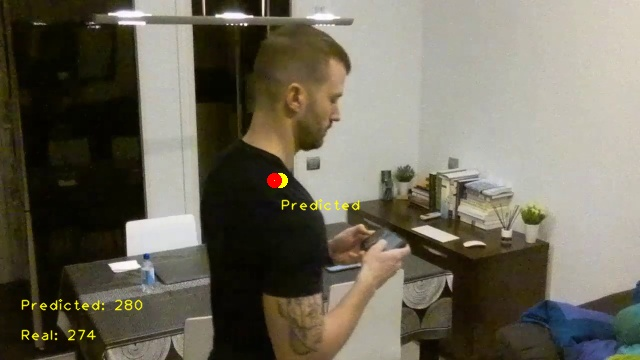
\includegraphics[width = 0.4\linewidth]{figuras/experiments/policy_gradient/test_images/33_real_274_predicted_280_actions_taken_4_pg_50epochs.jpg}}
	\hspace{0.05\linewidth}
	\subfloat[9 acciones tomadas]{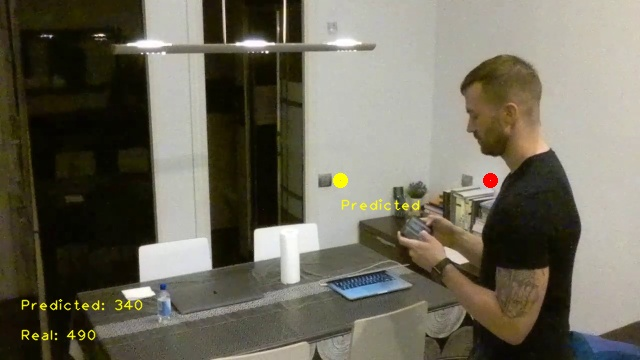
\includegraphics[width = 0.4\linewidth]{figuras/experiments/policy_gradient/test_images/34_real_490_predicted_340_actions_taken_9_pg_50epochs.jpg}}
	\hspace{0.05\linewidth}
	\subfloat[5 acciones tomadas]{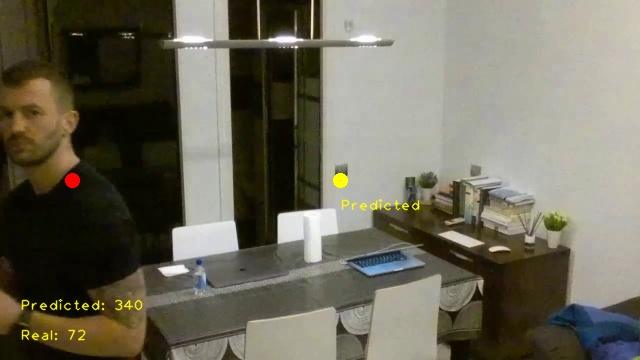
\includegraphics[width = 0.4\linewidth]{figuras/experiments/policy_gradient/test_images/53_real_72_predicted_340_actions_taken_5_pg_50epochs.jpg}}
	\hspace{0.05\linewidth}
	\subfloat[7 acciones tomadas]{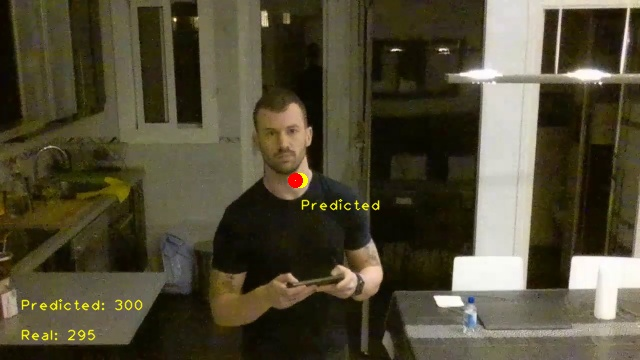
\includegraphics[width = 0.4\linewidth]{figuras/experiments/policy_gradient/test_images/87_real_295_predicted_300_actions_taken_7_pg_50epochs.jpg}}
    % \caption[Así aparece el rótulo en el índice]{Así aparece el rótulo en el texto.}
    \caption[Imágenes obtenidas en los experimentos usando \textit{Policy Gradient}]{Imágenes obtenidas en los experimentos usando \textit{Policy Gradient} sobre el conjunto de test}
    \label{fig-resultados-experimentos-policy-gradient}
\end{figure}

Por concluir, podemos decir que este primer conjunto de experimentos nos permitió entender la importancia de nuestra política de recompensa y resaltó problemas que no habíamos tenido en cuenta previamente en relación con las decisiones del agente.
\medskip


\section{Actor-Critic}
\label{resultados-actor-critic}

Usando los resultados previos con el algoritmo Policy Gradient, lo que buscamos con estos nuevos experimentos es obtener una mejora en cuanto a resultados y en cuanto a la estabilización de nuestro entrenamiento, gracias a la doble salida que obtiene nuestro agente, por un lado la distribución de probabilidad de las acciones a tomar y por otro lado el valor del estado en el que se encuentra.
\medskip

Para intentar evitar los problemas mencionados en los experimentos anteriores, en esta fase nos centramos ya no tanto en la búsqueda de los hiperparámetros correctos para el entrenamiento del agente, ya que usaremos las mismas técnicas utilizadas previamente, sino en refinar y construir un sistema de recompensa que se adecuase más al objetivo que queríamos lograr: llegar al punto objetivo con el menor de acciones posibles.
\medskip

\subsection{Experimento 1}
\label{resultados-actor-critic-experimento-1}

(temporal) Tensorboard: Actor-Critic-v2

Para este primer experimento, dejamos el sistema de recompensa previo, pero modificamos el número total de acciones por imagen, aumentándolo de 50 a 100.
\medskip

El entrenamiento se ejecutó durante 20 \textit{epochs}, basándonos en la convergencia obtenida en los experimentos anteriores y en el tiempo que conlleva.
\medskip

\begin{figure}[H]
	\centering
	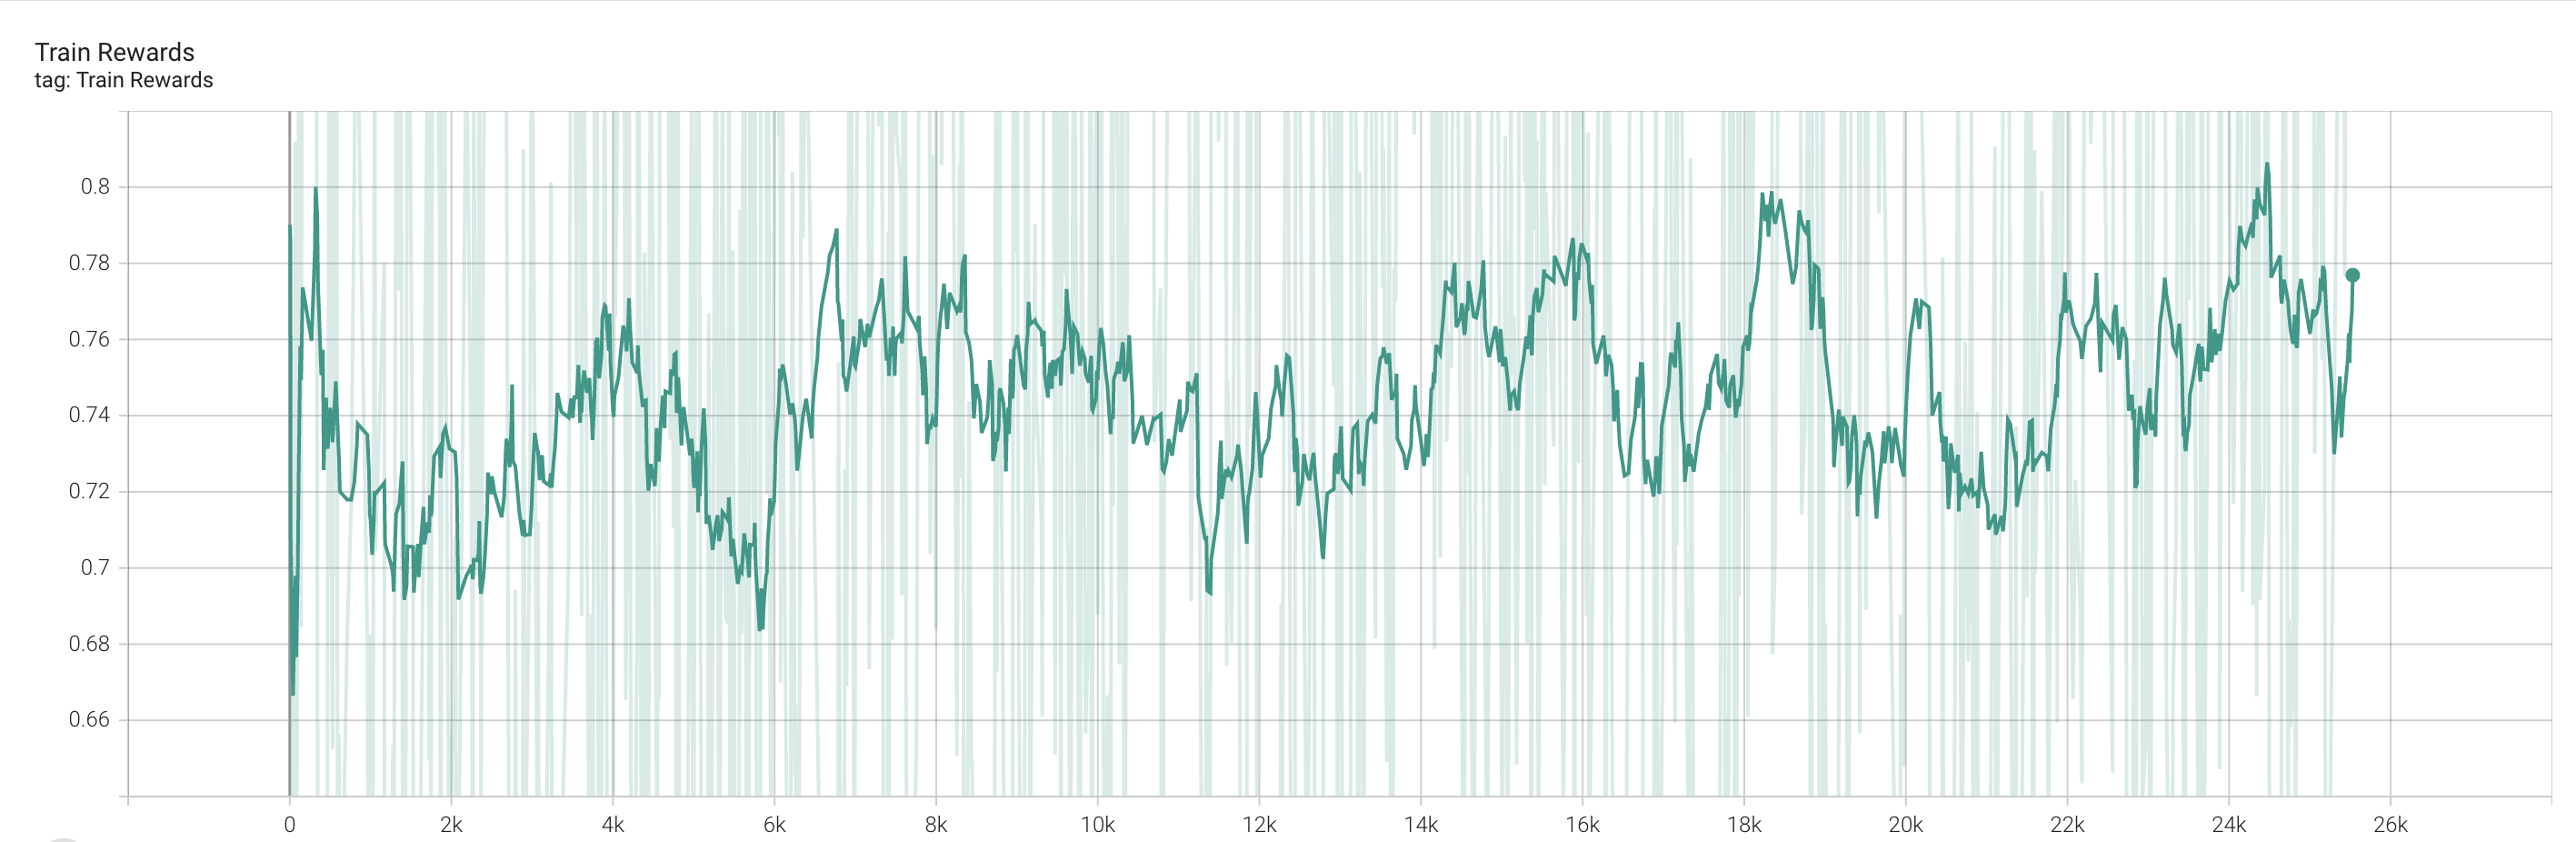
\includegraphics[width=1\textwidth]{figuras/experiments/actor_critic/actor_critic_20_epochs/train_rewards.png}
	\caption[Experimento Actor Critic 1 - Recompensa media en el conjunto de entrenamiento]{Experimento Actor Critic 1 - Recompensa media en el conjunto de entrenamiento}
	\label{fig-experimento-actor-critic-1-training-reward-mean}
\end{figure}
\begin{figure}[H]
	\centering
	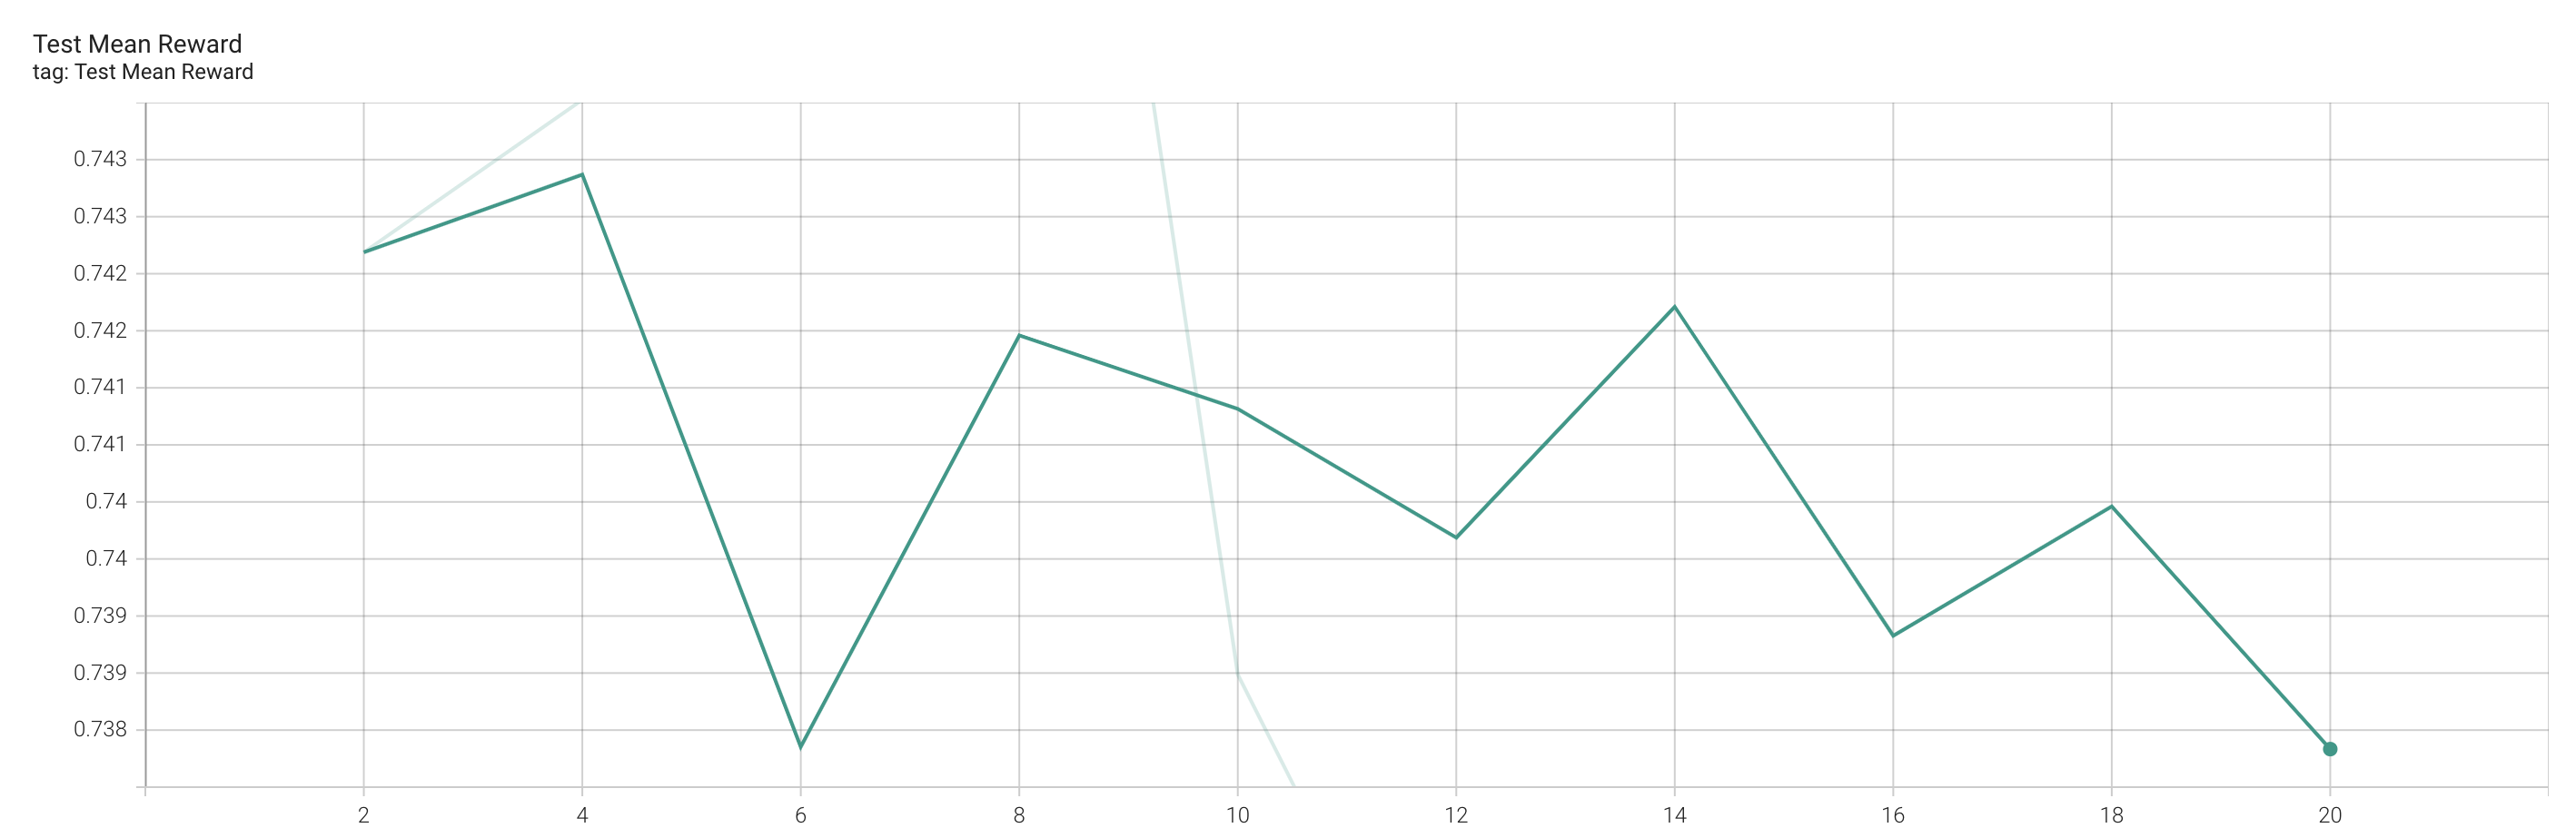
\includegraphics[width=1\textwidth]{figuras/experiments/actor_critic/actor_critic_20_epochs/test_mean_reward.png}
	\caption[Experimento Actor Critic 1 - Testing reward mean]{Experimento Actor Critic 1 - Testing reward mean}
	\label{fig-experimento-actor-critic-1-testing-reward-mean}
\end{figure}
\begin{figure}[H]
	\centering
	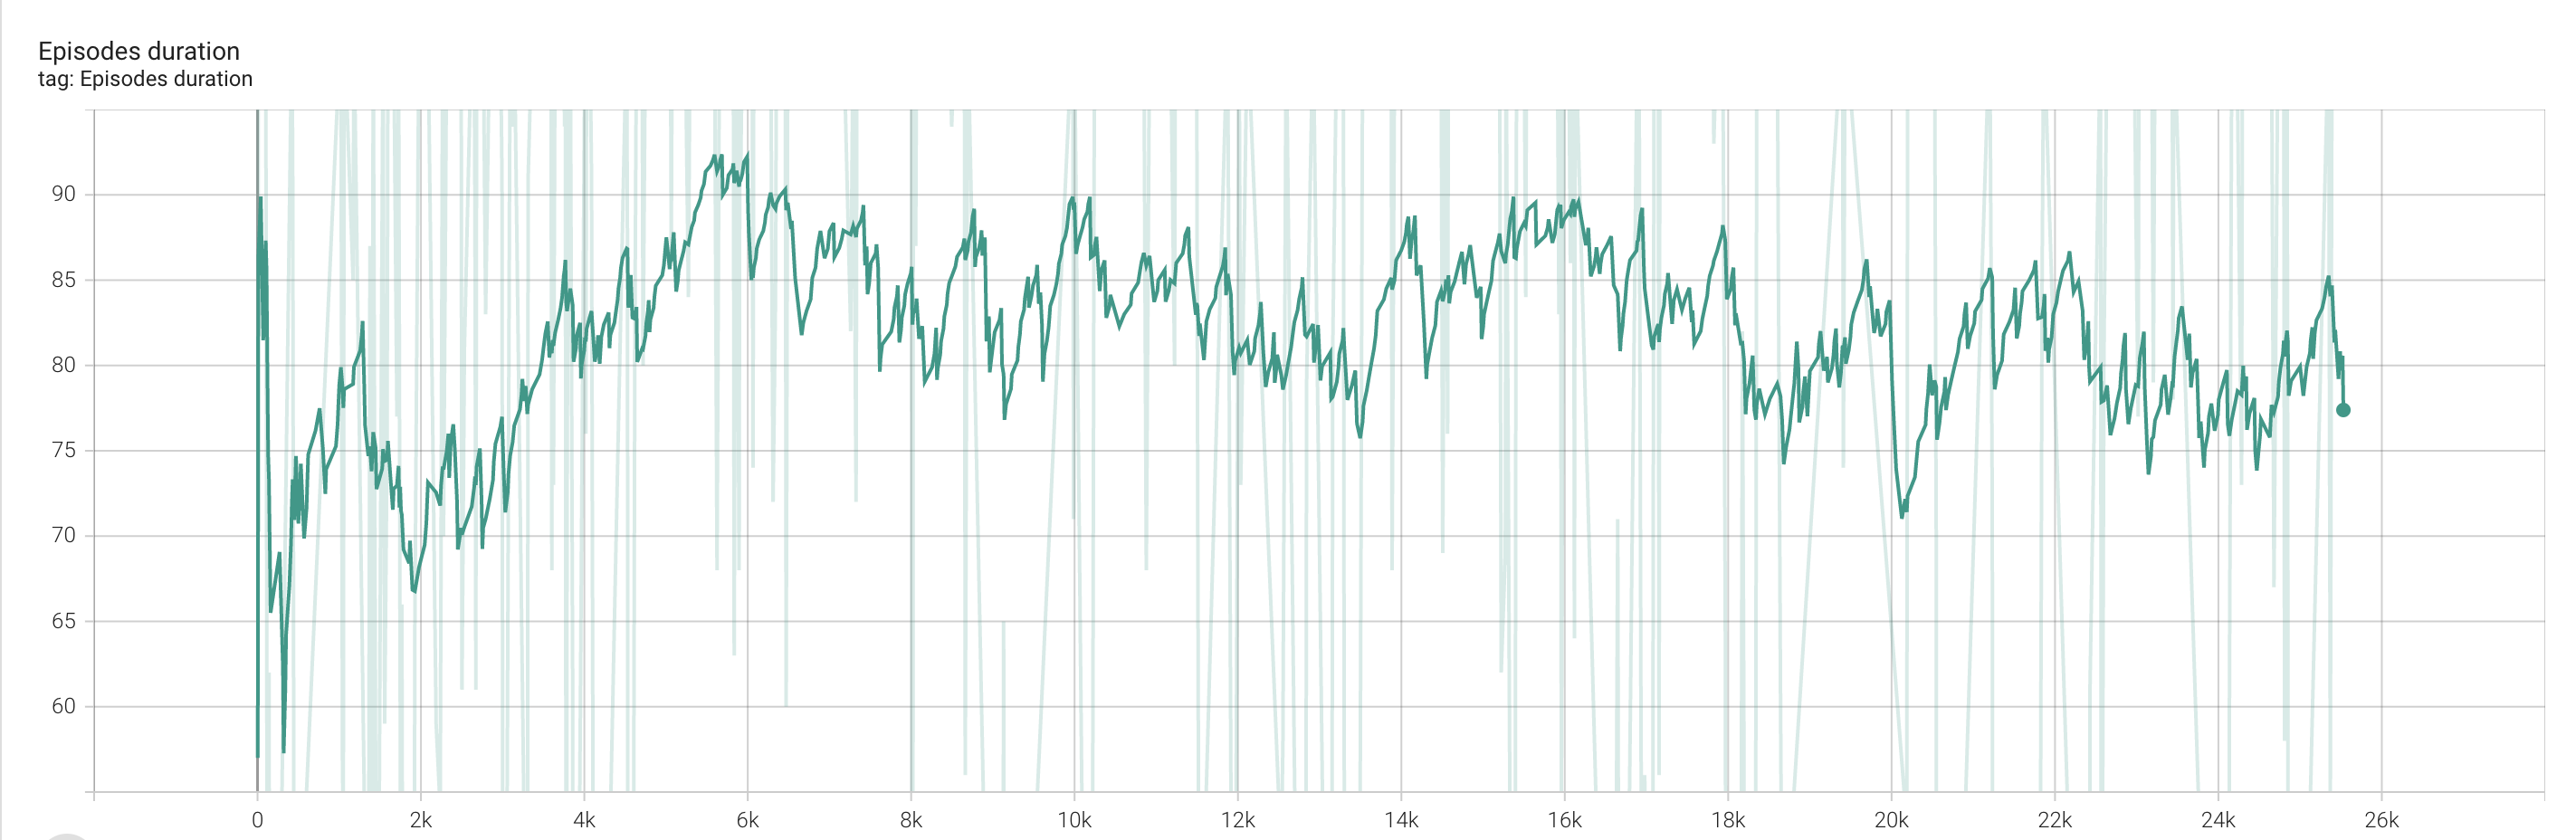
\includegraphics[width=1\textwidth]{figuras/experiments/actor_critic/actor_critic_20_epochs/episodes_duration.png}
	\caption[Experimento Actor Critic 1 - Duración de los episodios]{Experimento Actor Critic 1 - Duración de los episodios}
	\label{fig-experimento-actor-critic-1-episodes-duration}
\end{figure}
\begin{figure}[H]
	\centering
	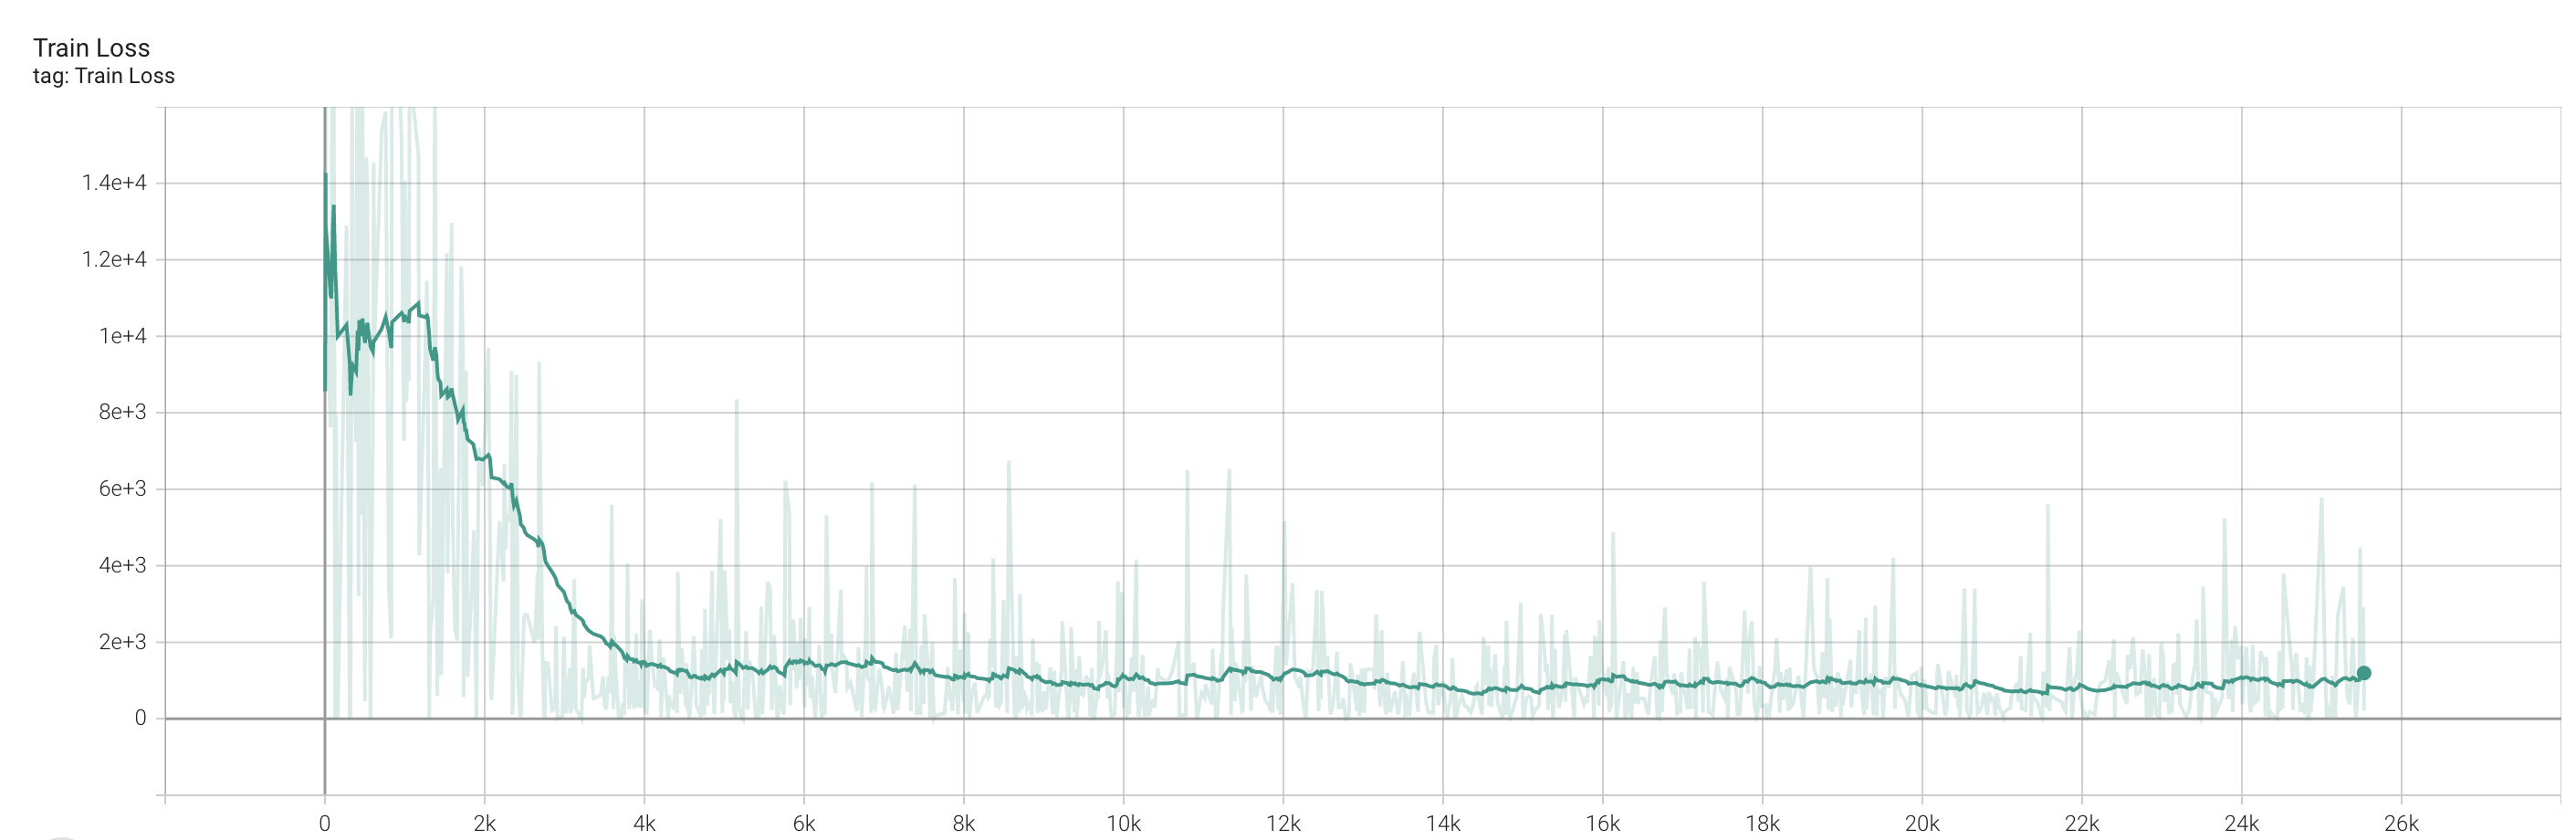
\includegraphics[width=1\textwidth]{figuras/experiments/actor_critic/actor_critic_20_epochs/train_loss.png}
	\caption[Experimento Actor Critic 1 - Train loss]{Experimento Actor Critic 1 - Train loss}
	\label{fig-experimento-actor-critic-1-train-loss}
\end{figure}
\medskip

Lo que podemos ver en este primer experimento es que, a pesar de nuestras expectativas inciales, el entrenamiento fue muy inestable, incluso más que en el caso de \textit{Policy Gradient}. Si bien se aprecia una tendencia a la alza en cuanto a la recompensa en el conjunto de datos de entrenamiento (figura \ref{fig-experimento-actor-critic-1-training-reward-mean}), vemos que no ocurre lo mismo en el conjunto de datos de test (fig. \ref{fig-experimento-actor-critic-1-testing-reward-mean}).
\medskip

Sin embargo, observamos que la función de coste en el entrenamiento desciende rápidamente y que se mantiene estable en un nivel bajo comparado con el inicial, lo cual nos hace sospechar de que el entrenamiento queda estancado a partir de ese punto, siendo esto un posible síntoma de que la red neuronal de nuestro agente no es lo suficientemente potente.
\medskip

\subsection{Experimento 2}
\label{resultados-actor-critic-experimento-2}

(temporal) (temporal) Tensorboard: Actor-Critic-ac-no-rewards-till-complete
Para este ejemplo decidimos incrementar el número de \textit{epochs}, de las 20 del experimento anterior hasta las 100, esperando que se produjese un salto en cuanto a la calidad del entrenamiento. Además disminuimos levemente el \textit{learning rate}.

\begin{figure}[H]
	\centering
	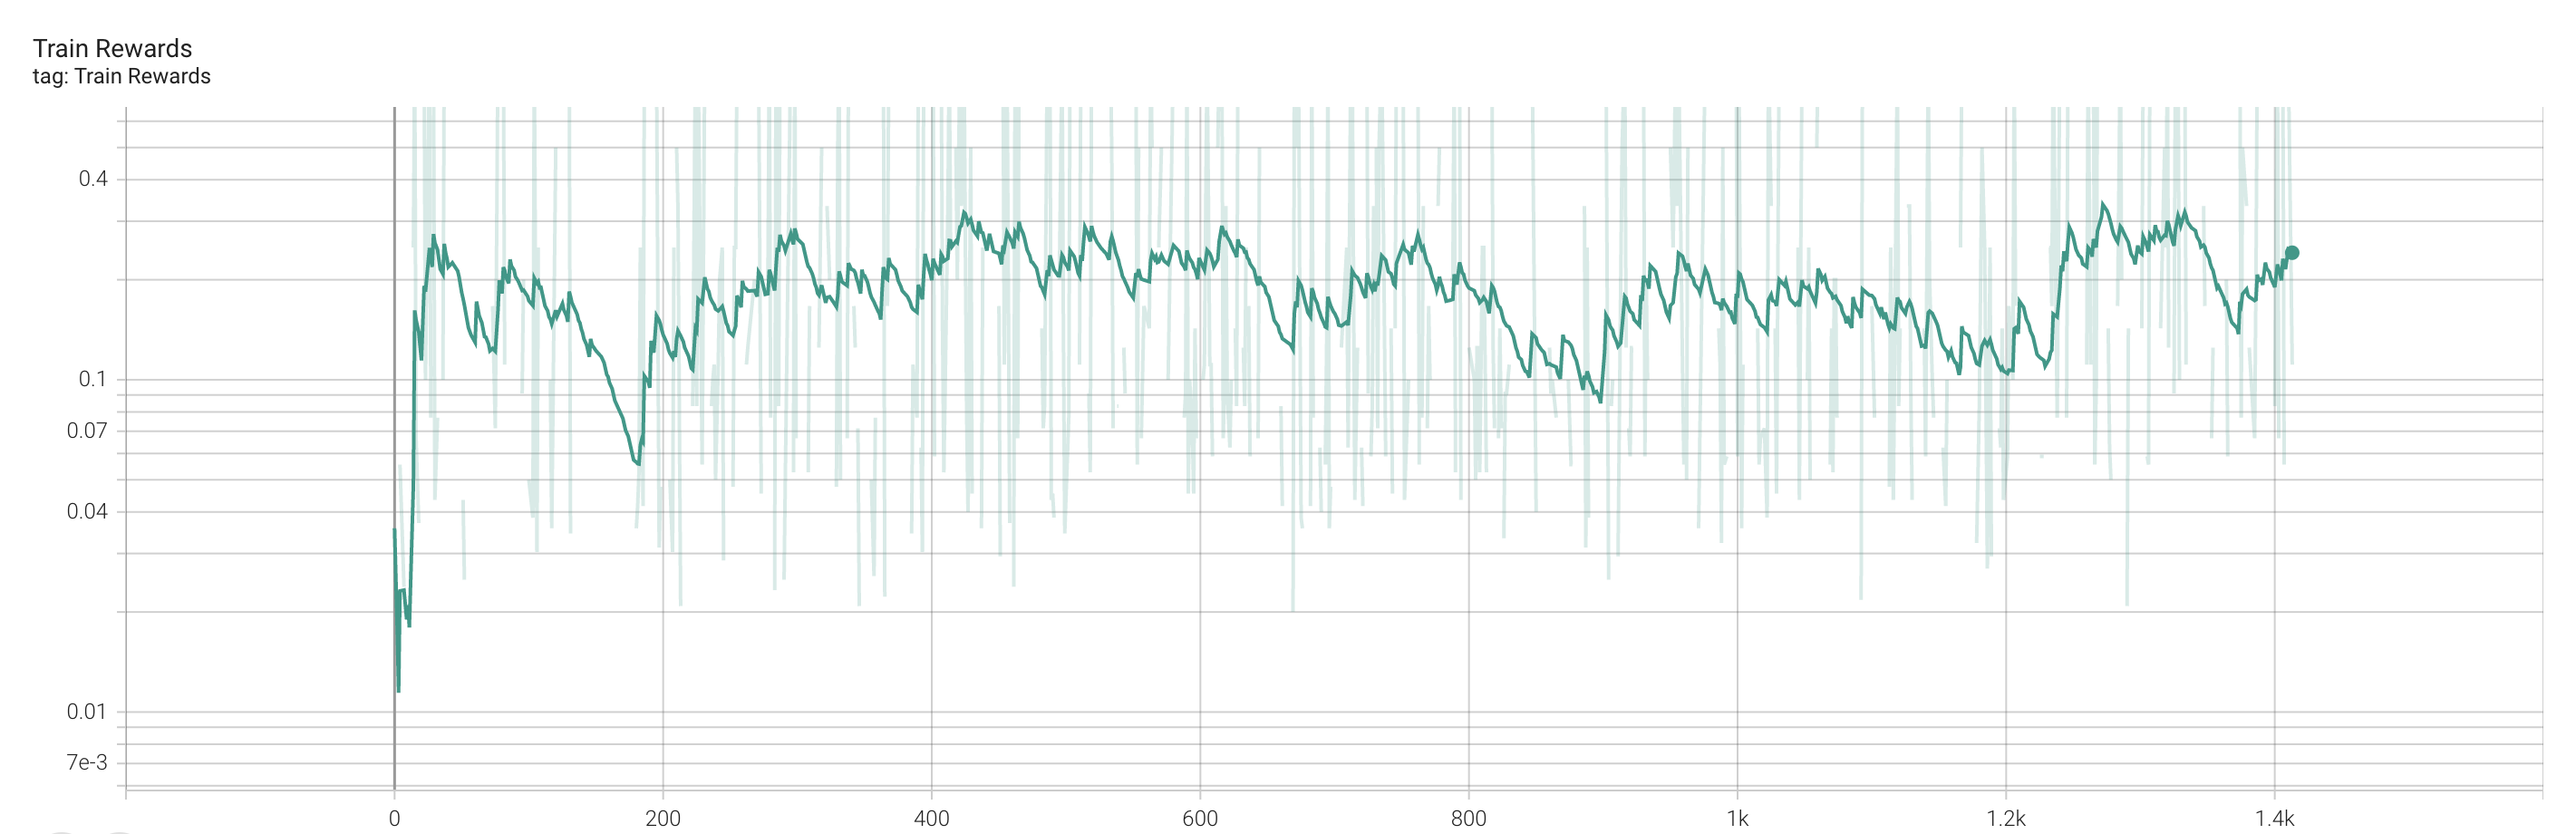
\includegraphics[width=1\textwidth]{figuras/experiments/actor_critic/actor_critic_no_rewards_till_complete/train_rewards.png}
	\caption[Experimento Actor Critic 2 - Recompensa media en el conjunto de entrenamiento]{Experimento Actor Critic 2 - Recompensa media en el conjunto de entrenamiento}
	\label{fig-experimento-actor-critic-2-training-reward-mean}
\end{figure}
\begin{figure}[H]
	\centering
	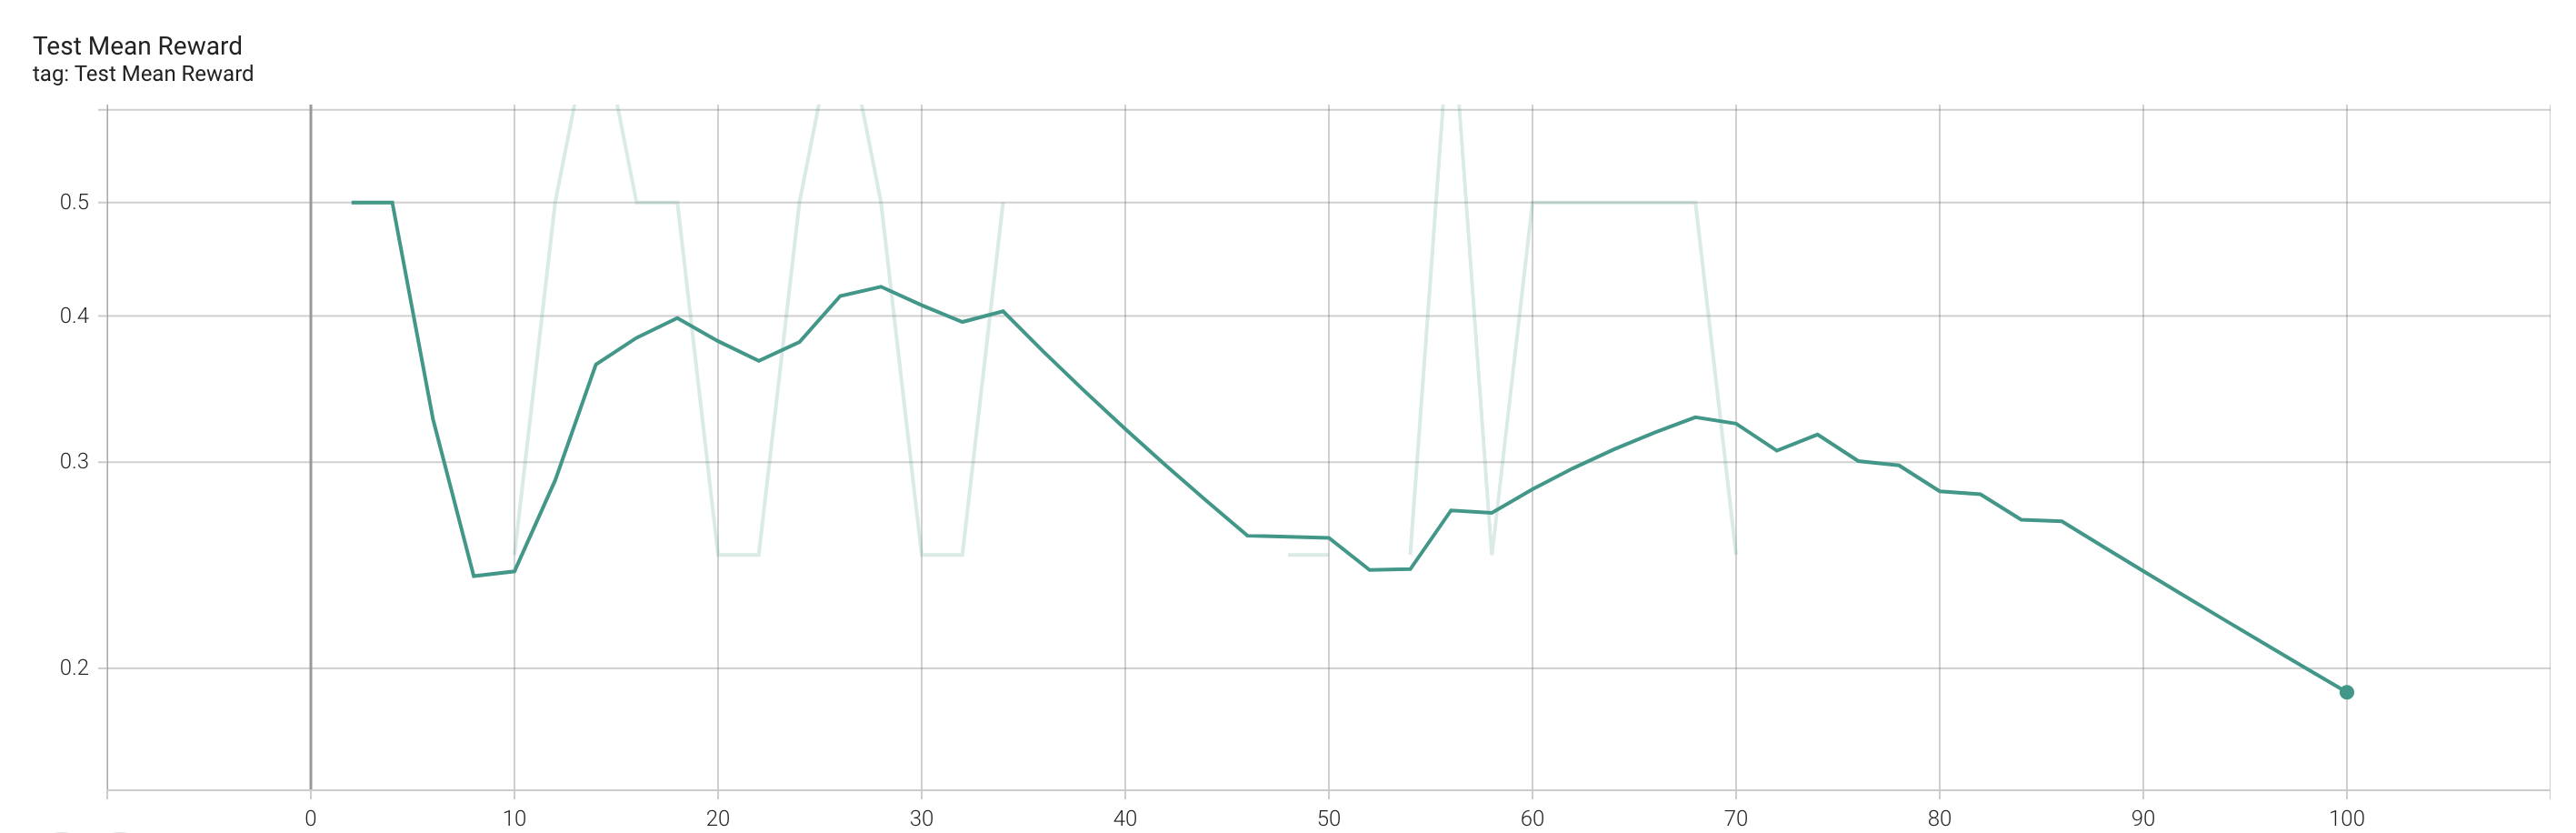
\includegraphics[width=1\textwidth]{figuras/experiments/actor_critic/actor_critic_no_rewards_till_complete/test_mean_reward.png}
	\caption[Experimento Actor Critic 2 - Testing reward mean]{Experimento Actor Critic 2 - Testing reward mean}
	\label{fig-experimento-actor-critic-2-testing-reward-mean}
\end{figure}
\begin{figure}[H]
	\centering
	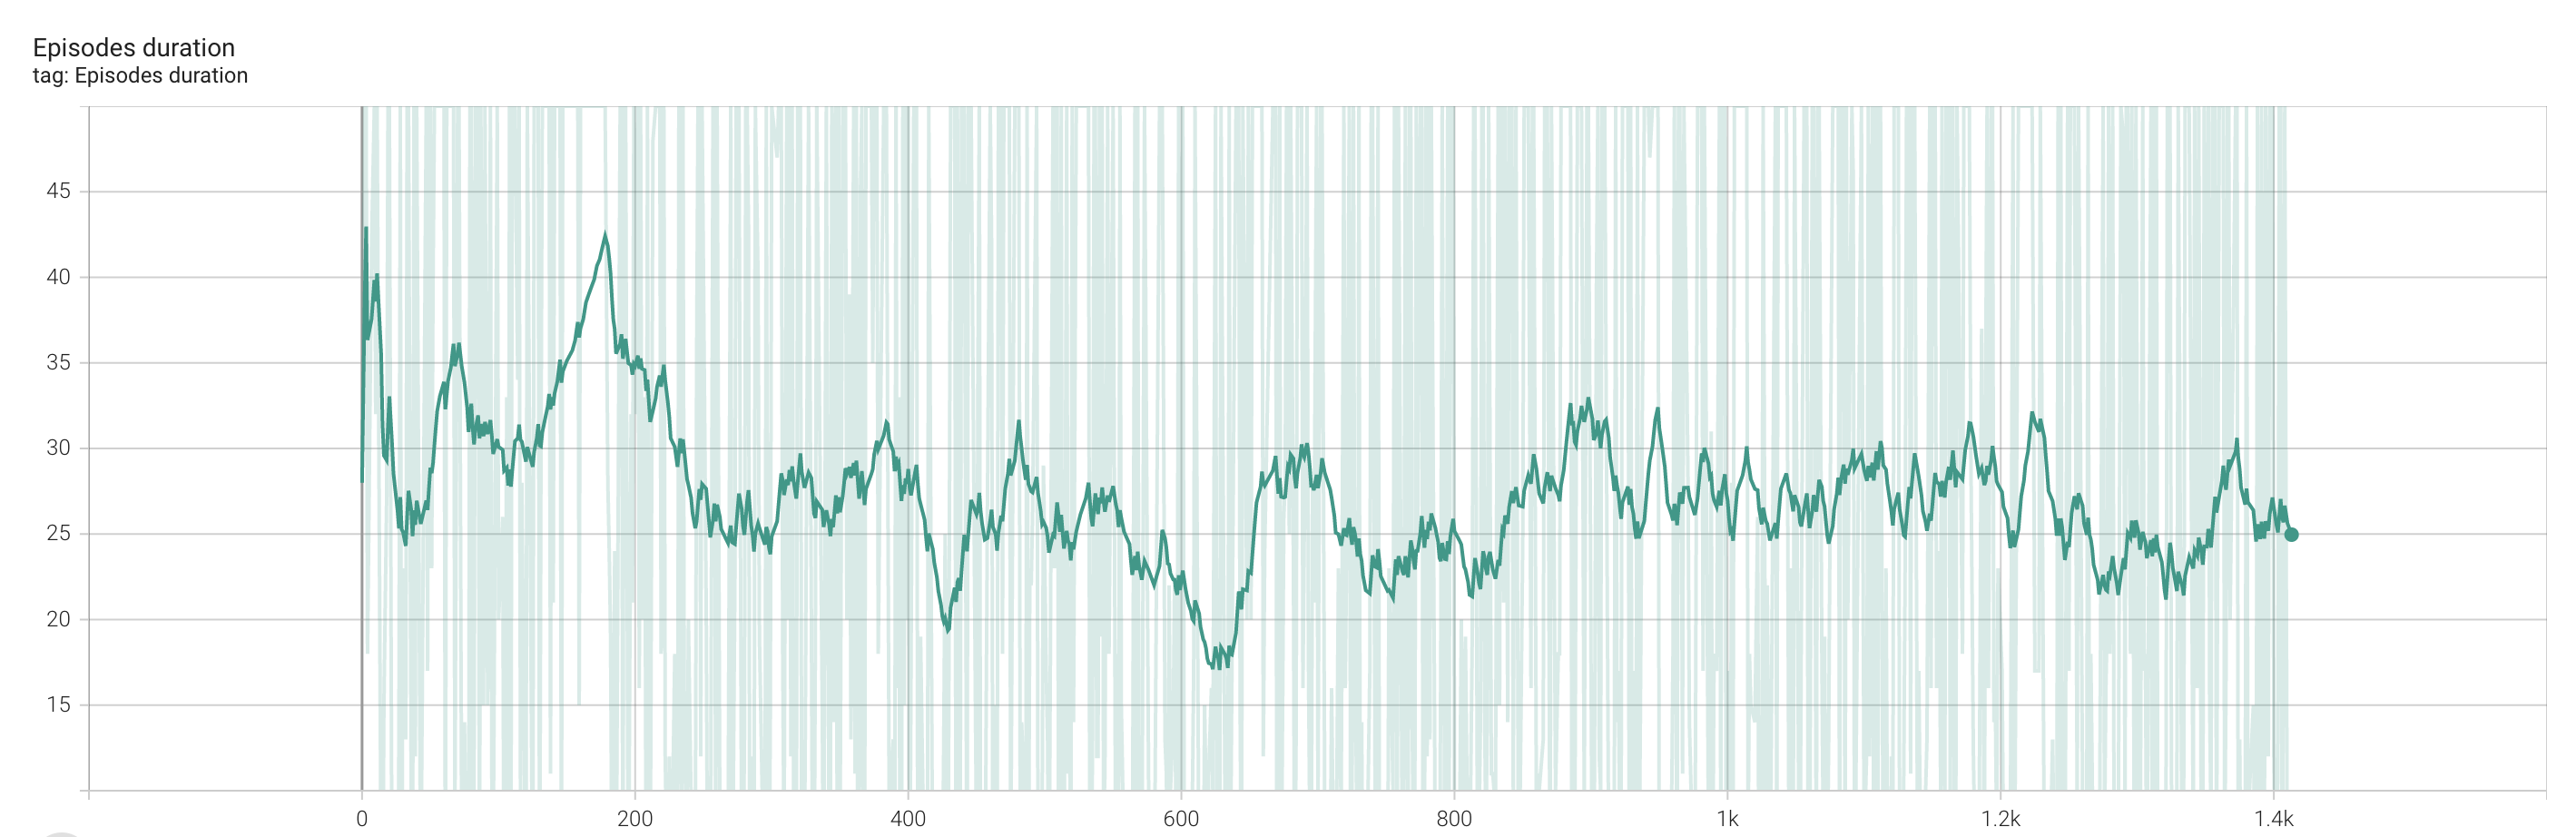
\includegraphics[width=1\textwidth]{figuras/experiments/actor_critic/actor_critic_no_rewards_till_complete/episodes_duration.png}
	\caption[Experimento Actor Critic 2 - Duración de los episodios]{Experimento Actor Critic 2 - Duración de los episodios}
	\label{fig-experimento-actor-critic-2-episodes-duration}
\end{figure}
\begin{figure}[H]
	\centering
	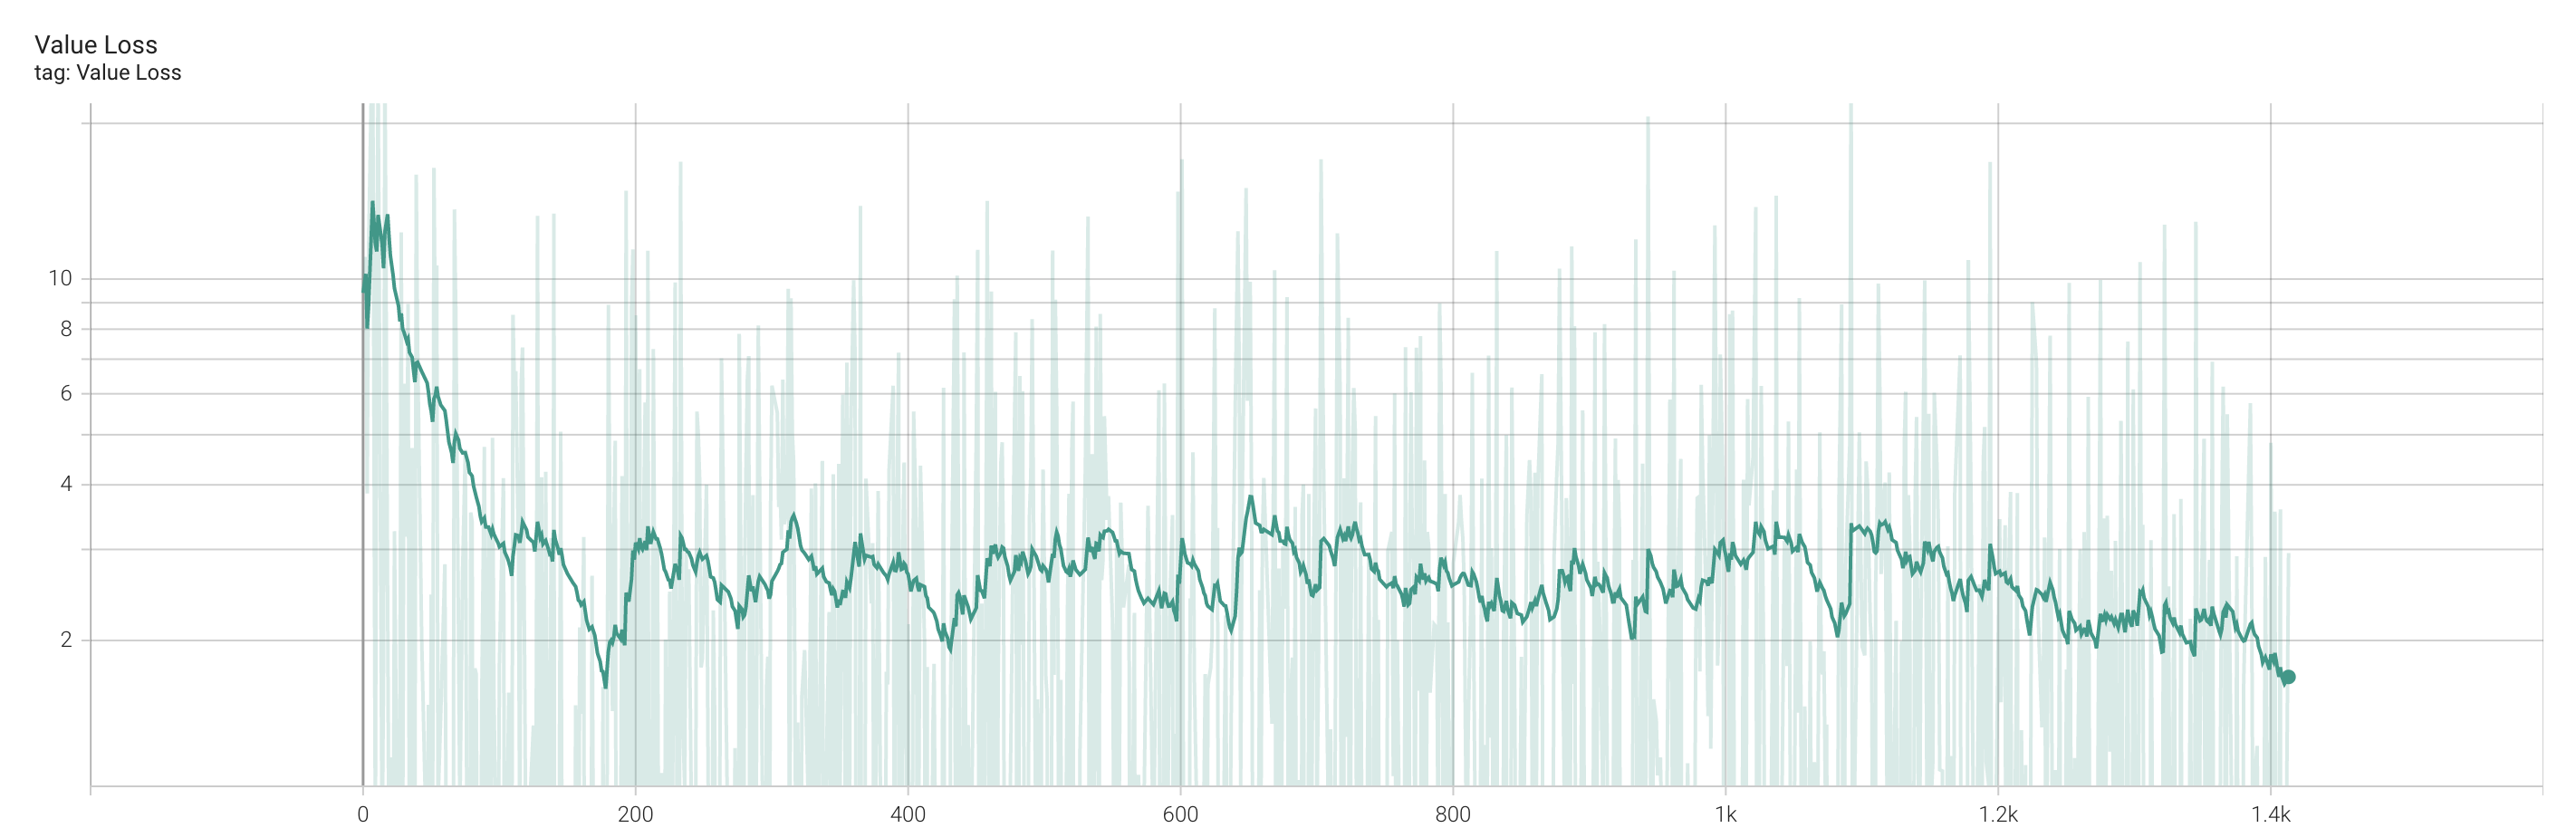
\includegraphics[width=1\textwidth]{figuras/experiments/actor_critic/actor_critic_no_rewards_till_complete/value_loss.png}
	\caption[Experimento Actor Critic 2 - Duración de los episodios]{Experimento Actor Critic 2 - Value loss}
	\label{fig-experimento-actor-critic-2-value-loss}
\end{figure}
\begin{figure}[H]
	\centering
	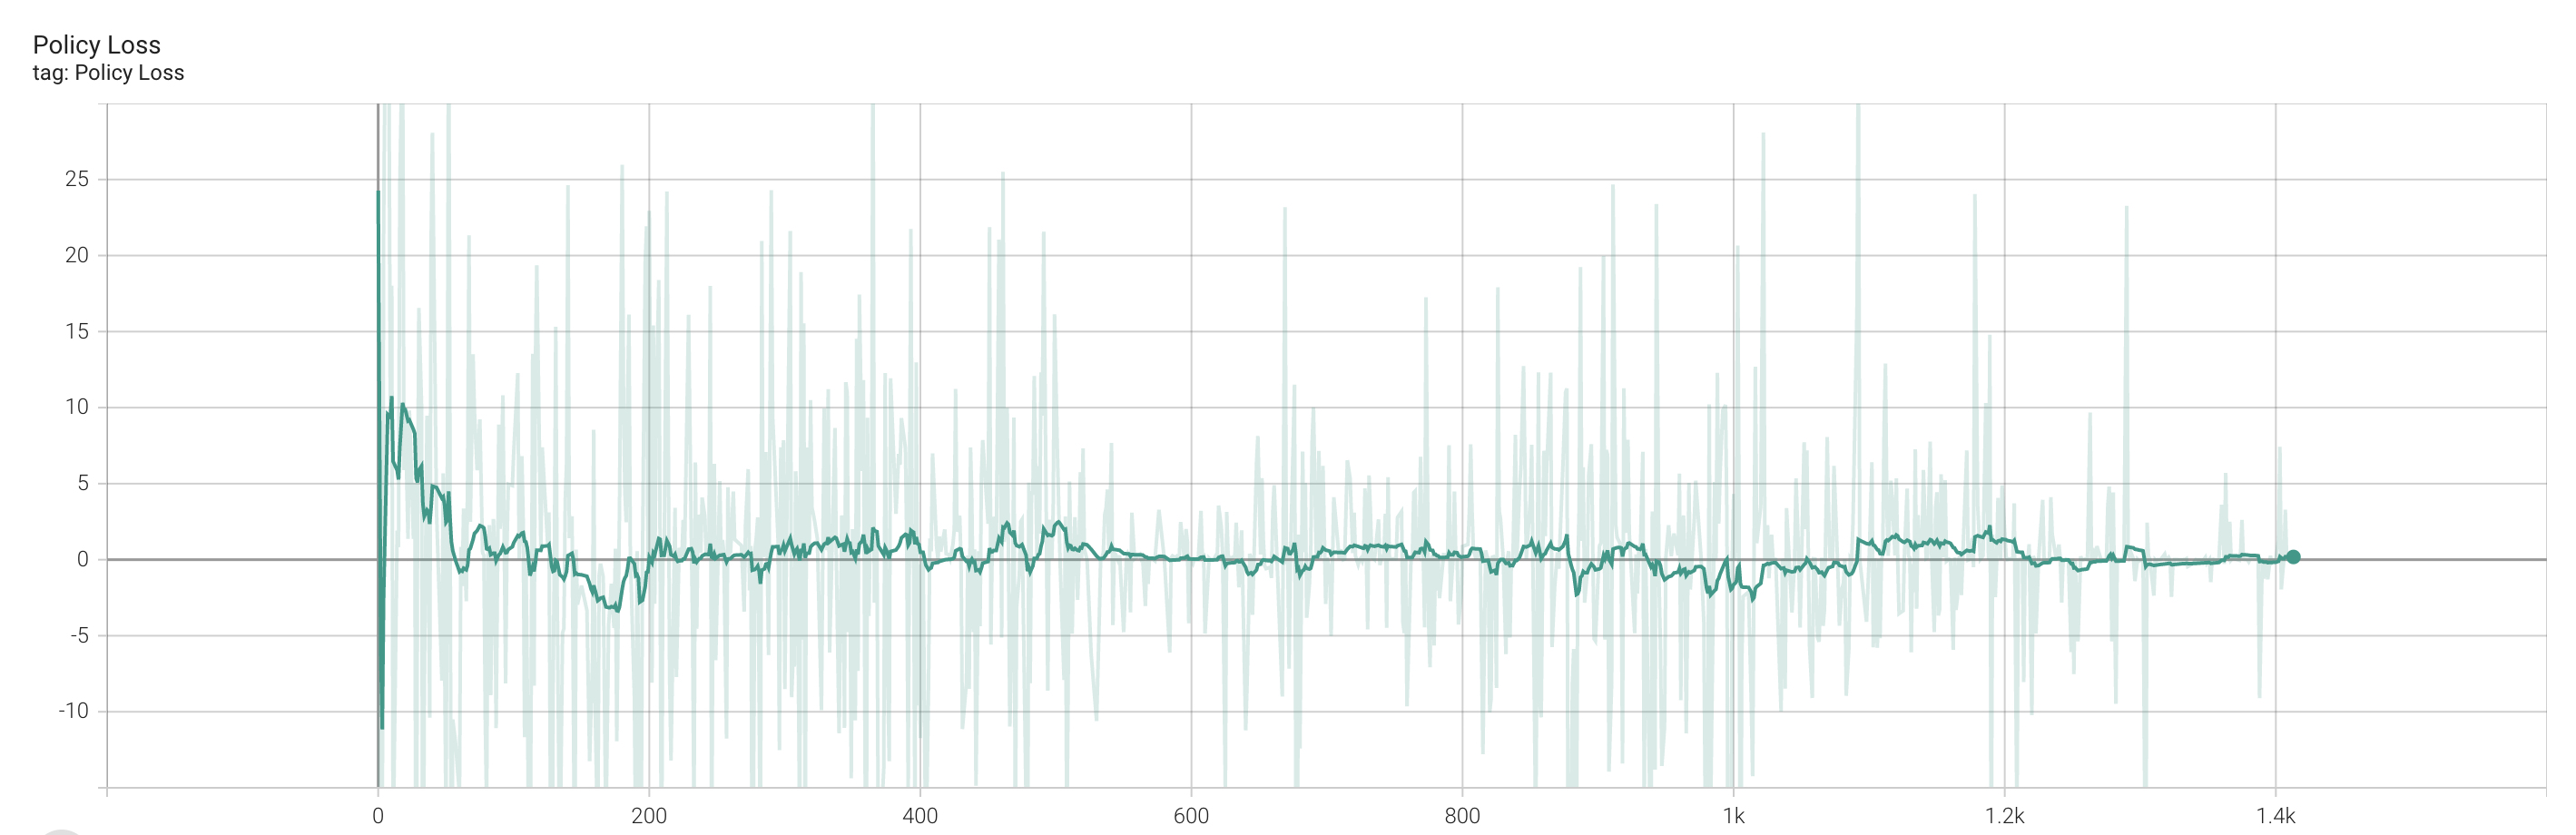
\includegraphics[width=1\textwidth]{figuras/experiments/actor_critic/actor_critic_no_rewards_till_complete/policy_loss.png}
	\caption[Experimento Actor Critic 2 - Duración de los episodios]{Experimento Actor Critic 2 - Policy loss}
	\label{fig-experimento-actor-critic-2-policy-loss}
\end{figure}

En este caso, cambiamos el sistema de recompensa al agente. Lo que hicimos fue darle una recompensa de 0 hasta que no llegase al final del episodio si es que no superaba el número de acciones máxima. La idea era reforzar aquellas experiencias en las que el agente tenía un resultado positivo y castigar aquellos intentos en los que no llegase al punto objetivo.
\medskip

Sin embargo, para disminuir la dificultad del episodio, lo que hicimos fue crear una zona de unos 30 píxeles tanto a la izquierda como a la derecha del punto objetivo, de manera que si el agente se acercaba por alguno de los lados, el episodio acabaría de manera satisfactoria.
\medskip

Al igual que en el experimento anterior, lo que podemos observar es que el agente aprende rápido durante las primeras iteraciones pero luego no se ve ninguna mejora significativa. En la figura \ref{fig-experimento-actor-critic-2-value-loss} vemos como la función de coste del agente si bien se mantiene prácticamente estable, va disminuyendo lentamente durante todo el entrenamiento, mientras que la \textit{policy loss} (fig. \ref{fig-experimento-actor-critic-2-policy-loss}) es prácticamente la misma.
\medskip

\subsection{Experimento 3}
\label{resultados-actor-critic-experimento-3}

(temporal) Tensorboard: Actor-Critic-ac-reward-2-rew-by-two-stop-with-none

En este experimento lo que haremos será intentar atacar varias situaciones que nos encontramos en experimentos anteriores. Entre ellas el problema que también comentamos durante el análisis de los experimentos con \textit{Policy Gradient} y es el hecho de que el agente decide permanecer quieto nada más comenzar el episodio cuando se ejecuta el conjunto de test, llevando por un lado a una rapida finalización de los episodios, pero limitando la opción de explorar más allá del punto inicial. Como comentamos en un principio, idealmente nuestro agente debería finalizar, o lo que es lo mismo, decidir no moverse cuando está seguro de que el punto en el que se encuentra es óptimo. Esta situación en particular se discutirá en el apartado \ref{resultados-conclusiones-actor-critic-experimentos}.
\medskip

Para ello, el sistema de recompensa fue modificado de la siguiente manera:

\begin{itemize}
	\item En el caso de que el agente haya llegado al punto objetivo, se le dará una recompensa de 2, en vez de 1 (se mantiene el mismo formato de recompensas parciales si no se llega al punto objetivo).
	\item Si el agente escoge la acción de permanecer quieto y no lo hace en el punto de recompensa máxima, la recompensa que obtiene para esa acción se divide entre 2.
\end{itemize}
\medskip

El objetivo de estas modificaciones es que el agente tenga una motivación extra por llegar al final del episodio dándole una recompensa extra en caso de que asi sea, lo que bajo nuestra hipótesis inicial incitaría a que el agente no decida detenerse nada más comenzar el episodio.
\medskip

El siguiente objetivo, relacionado directamente con el anterior, es desfavorecer la elección de permanecer quieto a no ser que el agente esté seguro de ello diviendo la recompensa que obtiene en dicha acción si no se encuentra en el punto esperado.
\medskip

\begin{figure}[H]
	\centering
	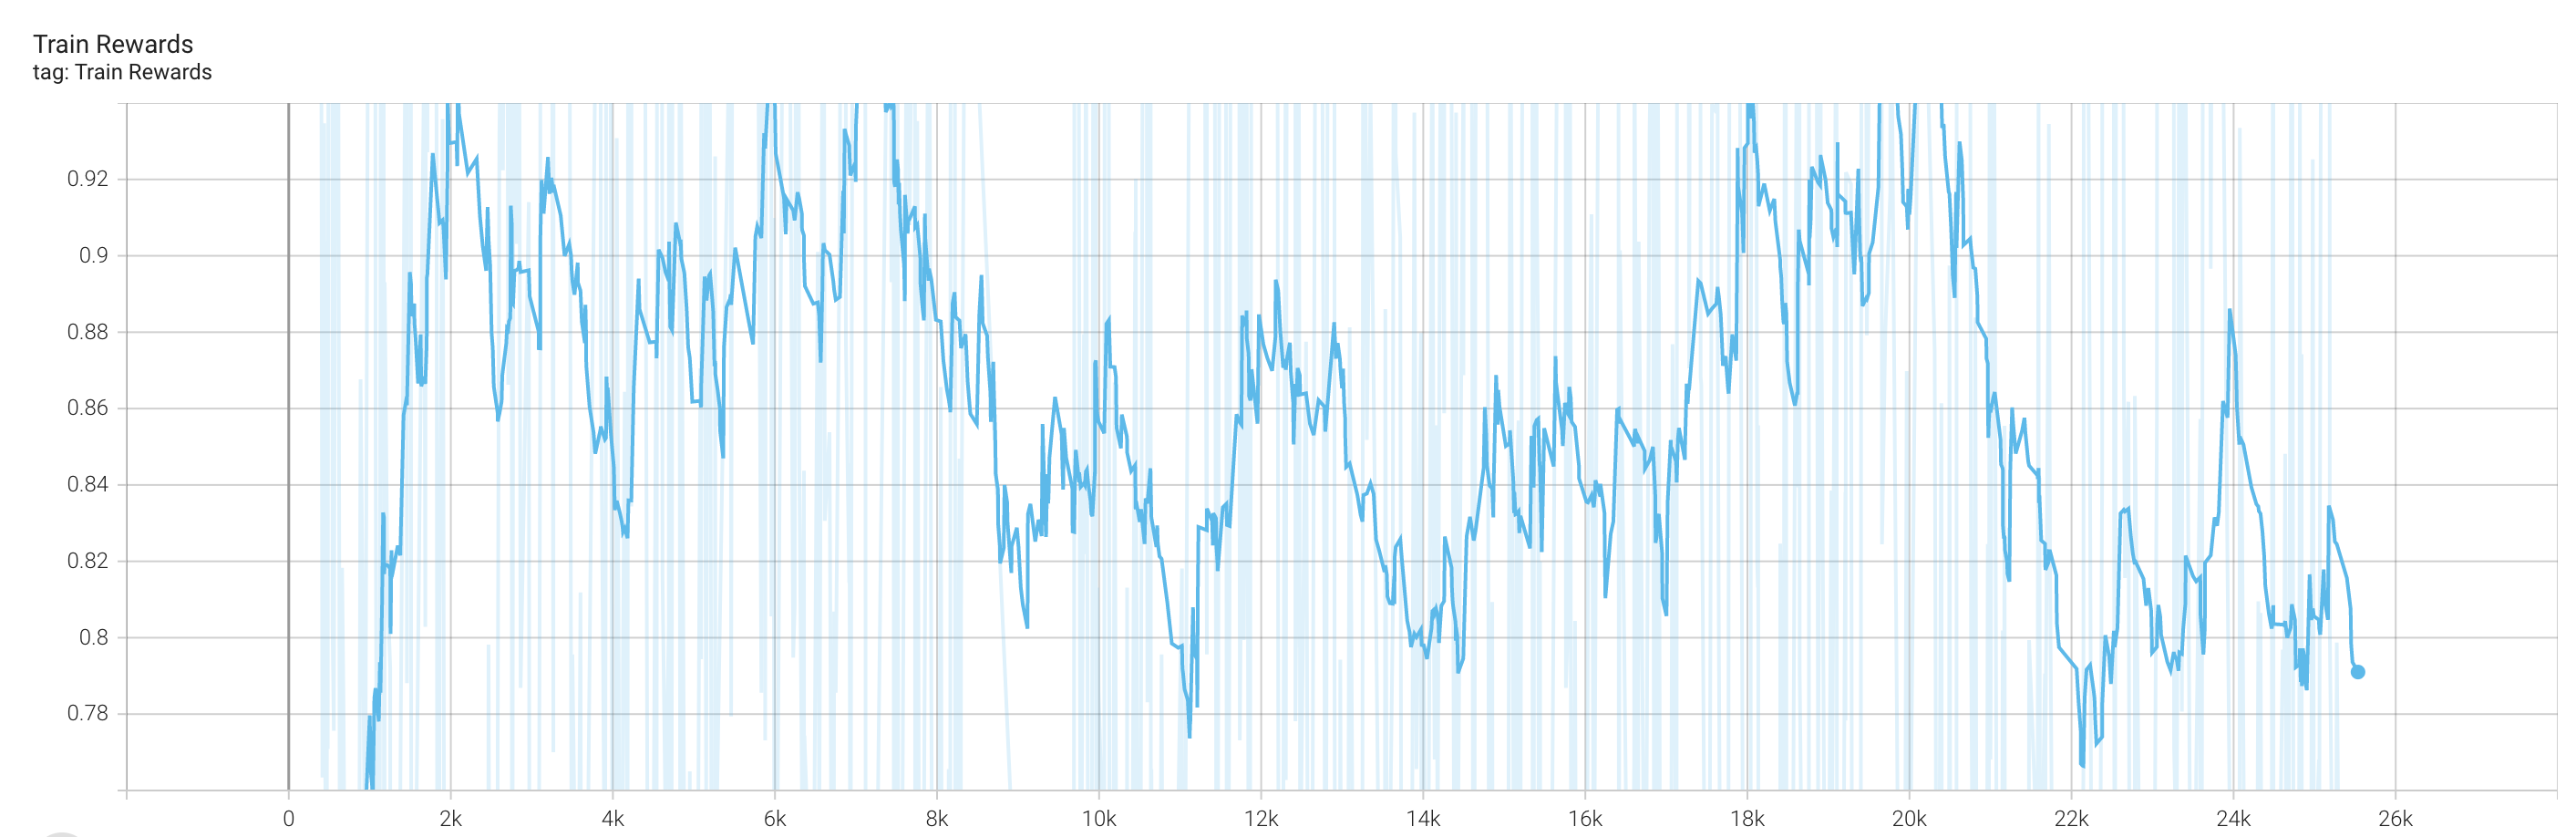
\includegraphics[width=1\textwidth]{figuras/experiments/actor_critic/reward_2_rew_by_two_stop_with_none/train_rewards.png}
	\caption[Experimento Actor Critic 3 - Recompensa media en el conjunto de entrenamiento]{Experimento Actor Critic 3 - Recompensa media en el conjunto de entrenamiento}
	\label{fig-experimento-actor-critic-3-training-reward-mean}
\end{figure}
\begin{figure}[H]
	\centering
	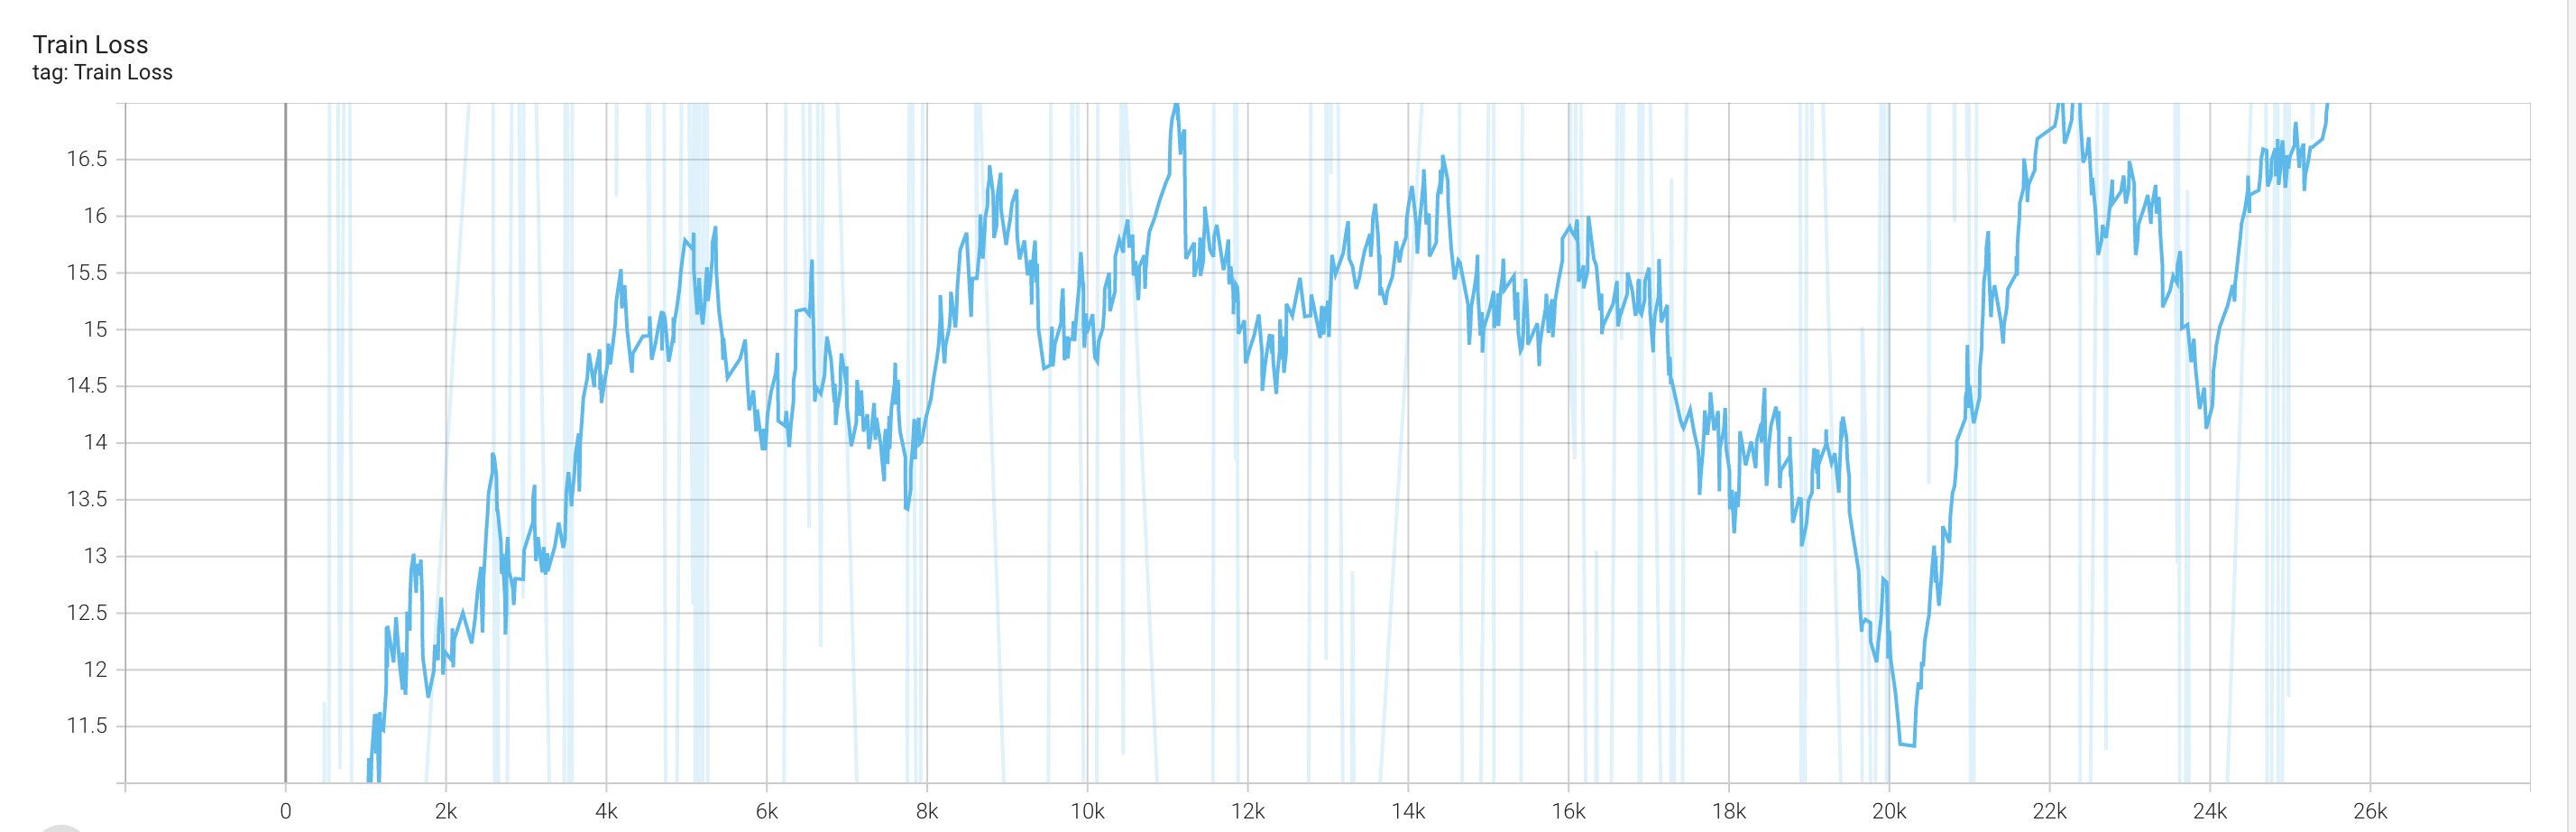
\includegraphics[width=1\textwidth]{figuras/experiments/actor_critic/reward_2_rew_by_two_stop_with_none/train_loss.png}
	\caption[Experimento Actor Critic 3 - Función de perdida]{Experimento Actor Critic 3 - Función de perdida}
	\label{fig-experimento-actor-critic-3-training-loss}
\end{figure}
\begin{figure}[H]
	\centering
	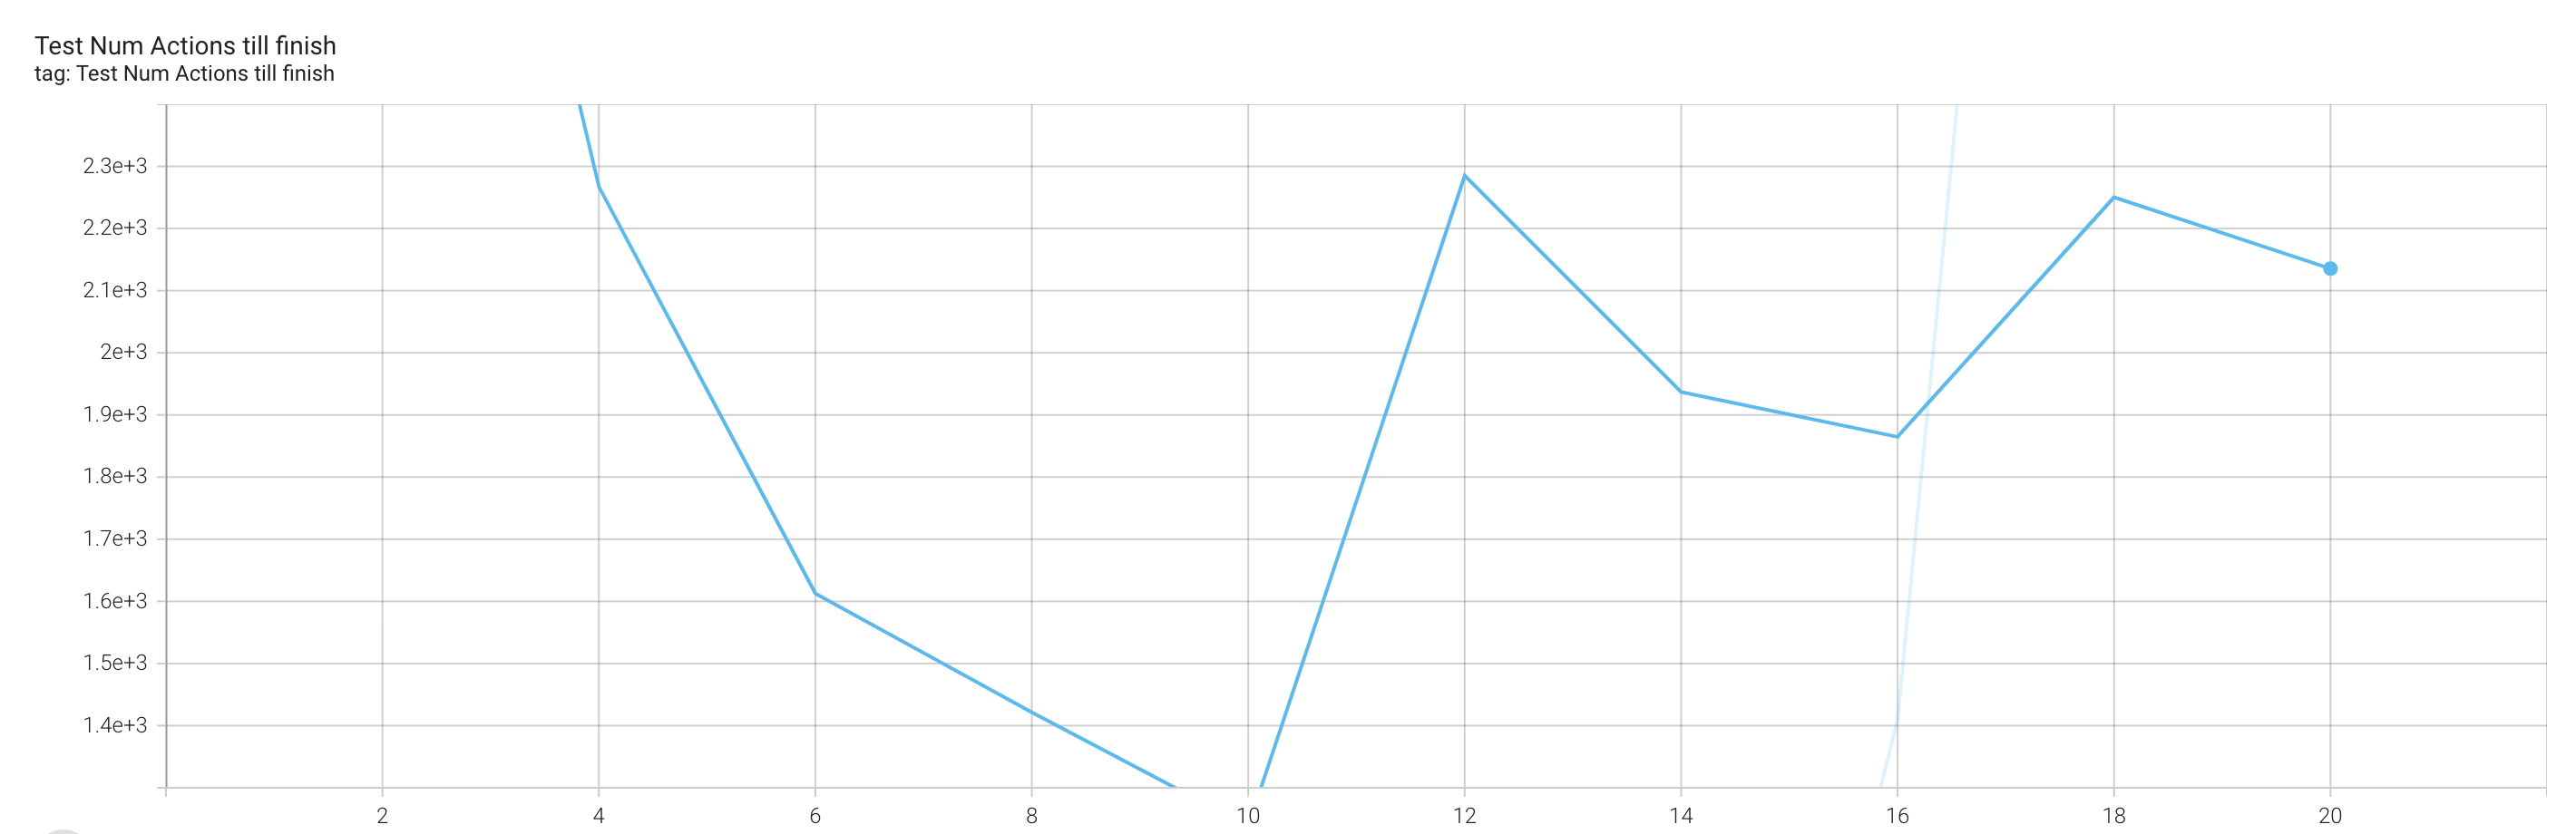
\includegraphics[width=1\textwidth]{figuras/experiments/actor_critic/reward_2_rew_by_two_stop_with_none/test_num_actions_till_finish.png}
	\caption[Experimento Actor Critic 3 - Número de acciones media por imagen]{Experimento Actor Critic 3 - Número de acciones media por imagen}
	\label{fig-experimento-actor-critic-3-testing-actions-till-finish}
\end{figure}
\begin{figure}[H]
	\centering
	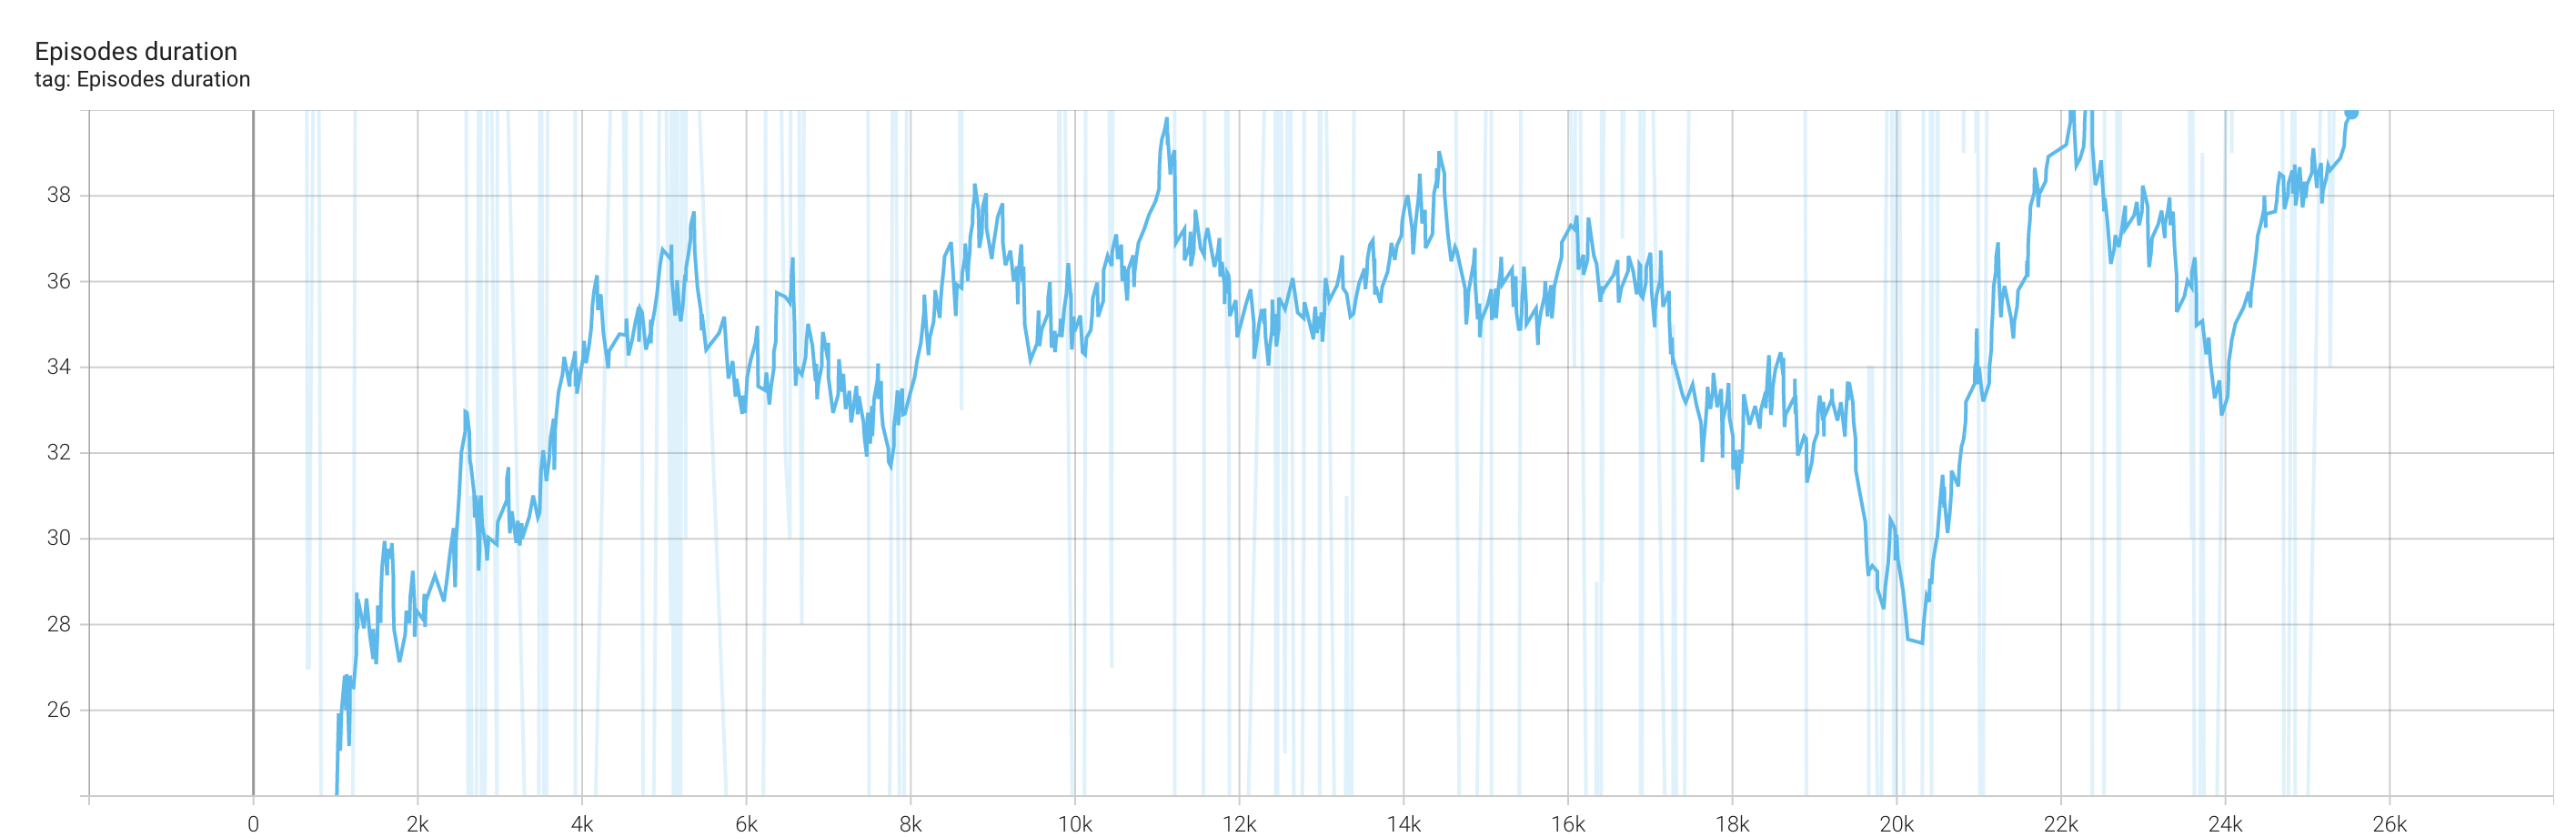
\includegraphics[width=1\textwidth]{figuras/experiments/actor_critic/reward_2_rew_by_two_stop_with_none/episodes_duration.png}
	\caption[Experimento Actor Critic 3 - Duración de los episodios]{Experimento Actor Critic 3 - Duración de los episodios}
	\label{fig-experimento-actor-critic-3-episodes-duration}
\end{figure}

Como podemos observar, los cambios aplicados sobre nuestro sistema de recompensa tuvo un gran impacto en el entrenamiento del agente. Si observamos la figura \ref{fig-experimento-actor-critic-3-training-reward-mean} vemos que la recompensa media no siguió una tendencia, sino que fue variando hasta llegar a un pico casi al final del entrenamiento para finalmente descender. En ese mismo punto vemos que la función de perdida en el conjnuto de entrenamiento disminuye (fig. \ref{fig-experimento-actor-critic-3-training-loss}), lo cual en general nos podría indicar un buen rendimiento de nuestro agente en ese punto.
\medskip

Durante este experimento, dados los cambios realizados sobre el \textit{reward}, nos pareció interesante realizar un seguimiento al número de acciones que el agente realizaba sobre las imágenes del conjunto de testeo, lo que se puede ver en la figura \ref{fig-experimento-actor-critic-3-testing-actions-till-finish}. Lo que observamos en la gráfica es que, si bien nuestro objetivo era incrementar la confianza del agente a la hora de tomar la acción de permanecer quieto, lo que conseguimos fue que el número de acciones por episodio en el conjunto de test se disparara sustancialmente, llegando practicamente a las 2000 acciones de media por imagen, lo que haría prácticamente inviable su despliegue en un entorno real. Este resultado nos lleva a pensar que nuestra hipótesis desarrollo una desconfianza en el agente a la hora de tomar la decisión de no moverse, lo que hace que prefiera moverse hacía la izquierda o hacía a la derecha.
\medskip

Esta tendencia queda confirmada cuando observamos el archivo de registro del experimento (disponible en el repositorio del proyecto) en el que muestra las acciones escogidas por el agente en cada imagen:

\begin{table}[ht!]
\centering
\resizebox{\textwidth}{!}{
\begin{tabular}{@{}ccccc@{}}
\toprule
\textbf{Época / Episodio} & \textbf{Moverse a la izquierda} & \textbf{Moverse a la derecha} & \textbf{Permanecer quieto} \\ \midrule
Época 0/ Episodio 65             & 10                  & 8                  & 4                                    \\ \midrule
Época 0/ Episodio 285             & 109                  & 37                  & 5                                    \\ \midrule
Época 1/ Episodio 675             & 77                  & 101                  & 0                                   \\ \midrule
Época 2/ Episodio 715             & 107                  & 94                  & 0                                    \\ \bottomrule
\end{tabular}
}
% \caption[Así aparece el rótulo en el índice]{Así aparece el rótulo en el texto.}
\caption[Resultados Actor Critic - Acciones escogidas por el agente durante el entrenamiento]{Acciones escogidas por el agente durante el entrenamiento}
\label{table-numero-acciones-ejecucion}
\end{table}
% Epoch 0 Episode 65 Left:10 	 Right: 8	 None: 4
% Epoch 0 Episode 285 Left:109 	 Right: 37	 None: 5
% Epoch 1 Episode 675 Left:77 	 Right: 101	 None: 0
% Epoch 2 Episode 715 Left:107 	 Right: 94	 None: 0	


Al principio del entrenamiento el agente comienza tomando acciones aleatorias, lo cual es esperable debido a que no tiene experiencias previas con el entorno. Según va avanzando su conocimiento, vemos que incluso ya durante la primera época, el agente aprende a relacionar la acción de no moverse con una recompensa negativa y por lo tanto decide cada vez con mayor frecuencia no usarla, lo cual implica disminuir la probabilidad de esa acción en particular. Al cabo de la primera época ya observamos que la acción prácticamente ya no es escogida, lo cual nos lleva a confirmar nuestra teoría de que nuestro nuevo sistema de recompensa no está produciendo los resultados esperados.
\medskip

La investigación alrededor de este problema fue un punto clave en el desarrollo del proyecto y fue lo que nos llevó a probar diferentes alternativas no solo en cuanto al sistema de recompensa/castigo, probando con diferentes opciones como castigar al agente si el número de acciones era demasiado bajo o penalizar la trayectoria del episodio si no se terminó este con la recompensa máxima, sino también a explorar diferentes criterios de parada en el episodio.
\medskip

En lo relativo a los criterios de parada se decidió también probar como condición que fuese la propia acción de no moverse en lugar de la obtención de la recompensa máxima, junto con el número máximo de acciones por imagen para evitar un bucle infinito en el entrenamiento.
\medskip


\subsection{Experimento 4 - Vision Transformers}
\label{resultados-actor-critic-vision-transformers}

Para finalizar con esta sección de experimentos, decidimos incluir nuestro intento usando Vision Transformers como parte del preprocesamiento de la imagen. Esto a su vez involucró una transformación de la salida del Transformer a la capa de entrada de nuestro agente. Esto se realizó utilizando una red neuronal intermedia, ya que nuestro agente inicialmente recibía un vector con 4097 elementos como entrada y la salida del Transformer era una matriz de 197x512 elementos.
\medskip

Lo que intentábamos buscar con este experimento era el poder descartar la posibilidad de que la representación de nuestra imagen no fuese lo suficientemente característica para que nuestro agente pudiese distinguir qué era lo importante y que no. 
\medskip

Debido a la carga computacional de este modelo y las restricciones en cuanto a tiempo, no se pudieron realizar múltiples experimentos con la misma facilidad que antes. Sin embargo, nos sirvió para explorar e investigar otras soluciones, y aunque esta no fue la unica solución que tuvimos en cuenta, nos pareció interesante considerarla en la memoria debido a la popularidad que este tipo de redes cuentan a día de hoy y de la posibilidad de introducirlas en un problema de aprendizaje por refuerzo.
\medskip

\begin{figure}[H]
	\centering
	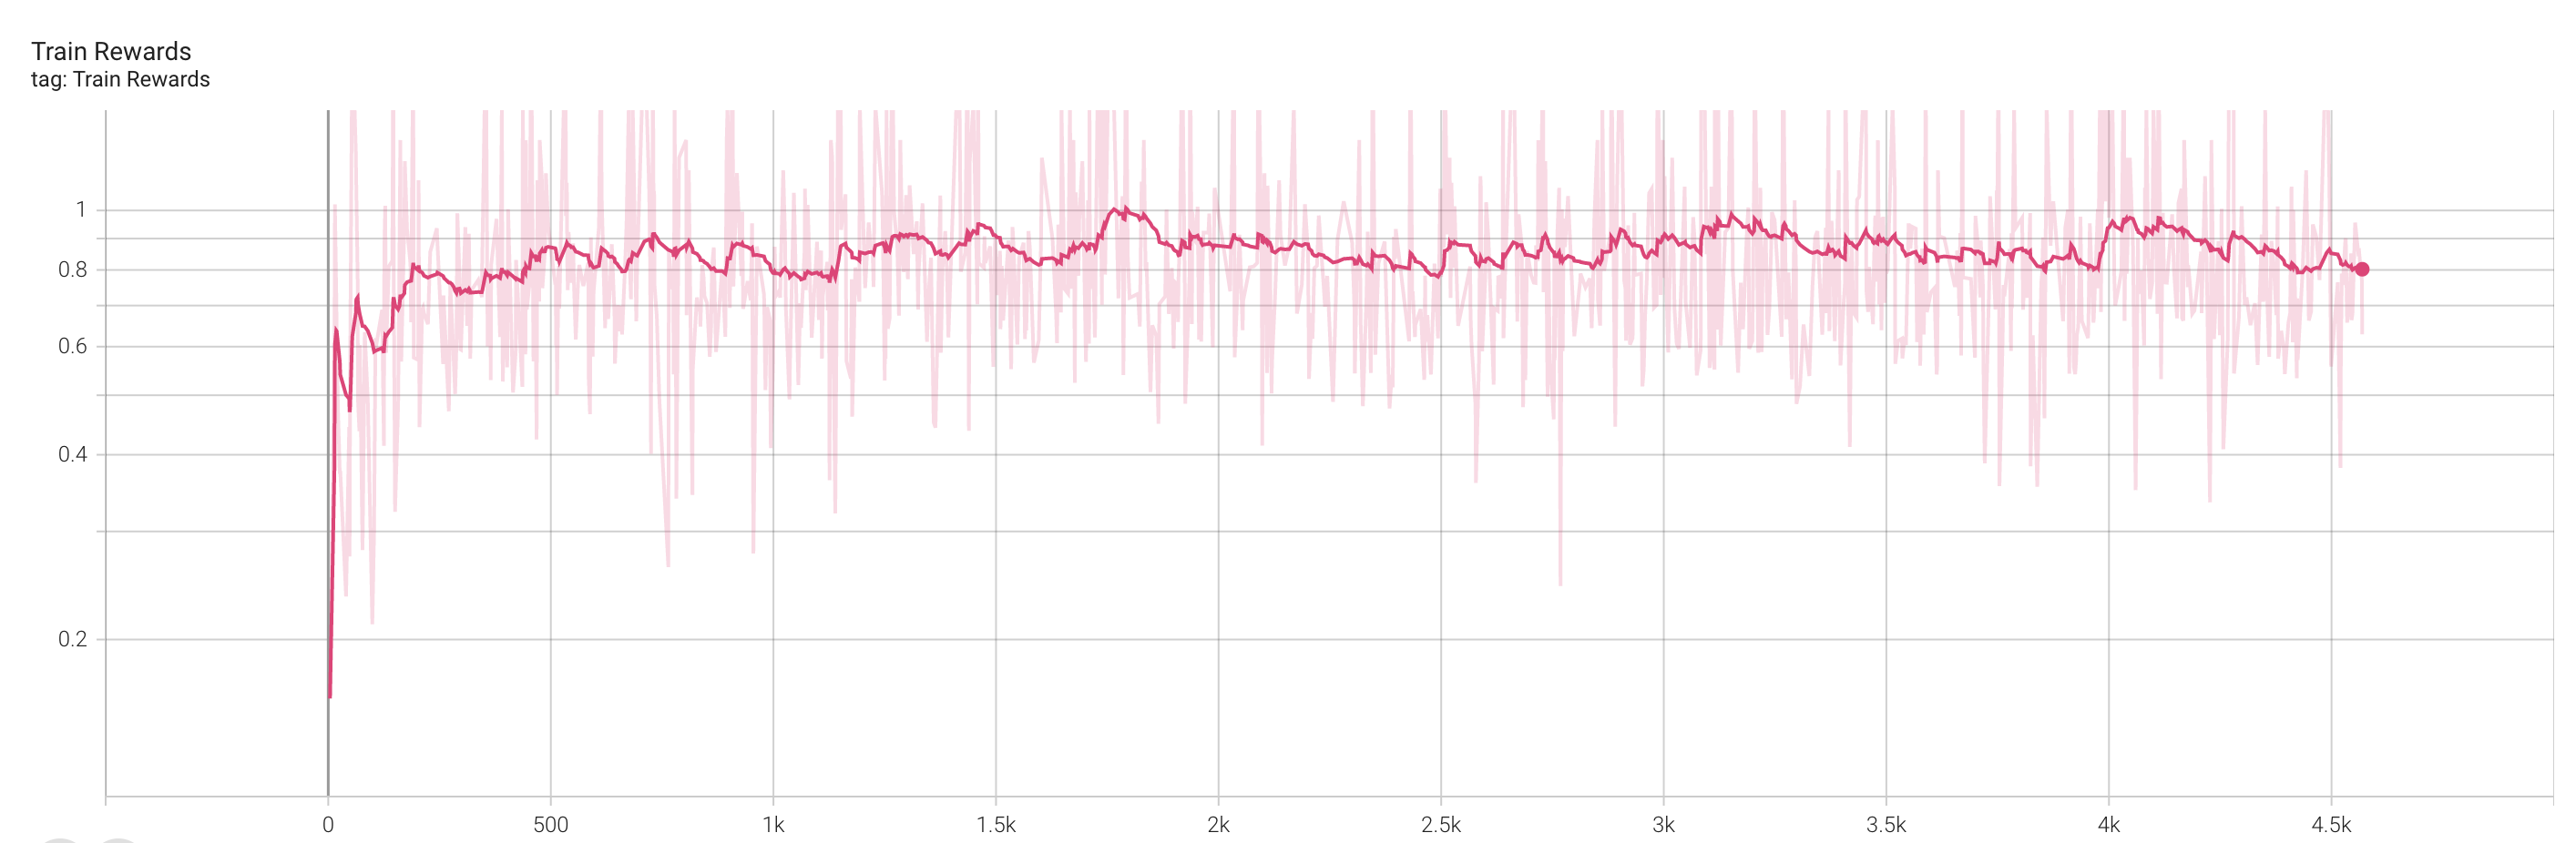
\includegraphics[width=1\textwidth]{figuras/experiments/vision transformers/train_rewards.png}
	\caption[Experimento \textit{Vision Transformer} - Recompensa media en el conjunto de entrenamiento]{Experimento \textit{Vision Transformer} - Recompensa media en el conjunto de entrenamiento}
	\label{fig-experimento-vision-transformer-1-training-reward-mean}
\end{figure}
\begin{figure}[H]
	\centering
	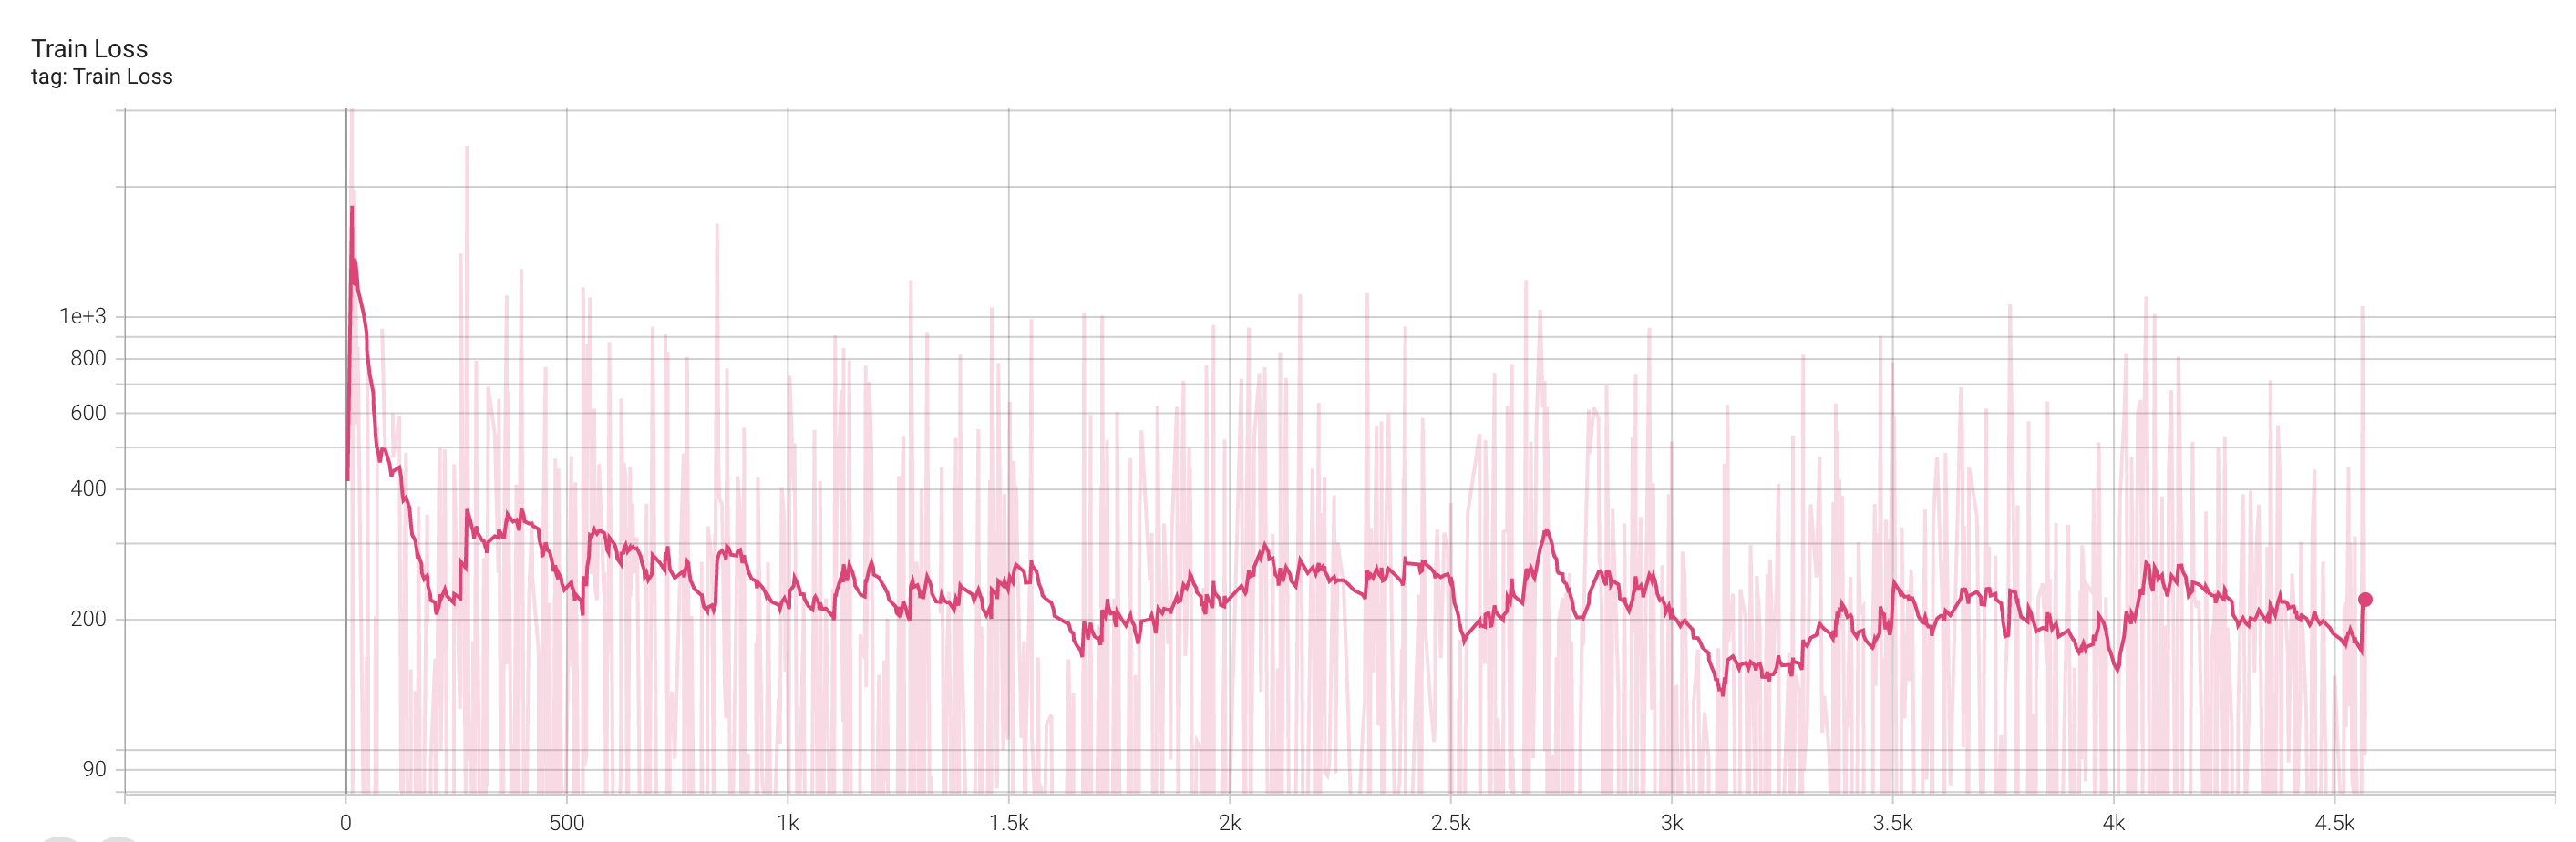
\includegraphics[width=1\textwidth]{figuras/experiments/vision transformers/train_loss.png}
	\caption[Experimento \textit{Vision Transformer} - Función de perdida en el conjunto de entrenamiento]{Experimento \textit{Vision Transformer} - Función de perdida en el conjunto de entrenamiento}
	\label{fig-experimento-vision-transformer-1-training-loss}
\end{figure}
\begin{figure}[H]
	\centering
	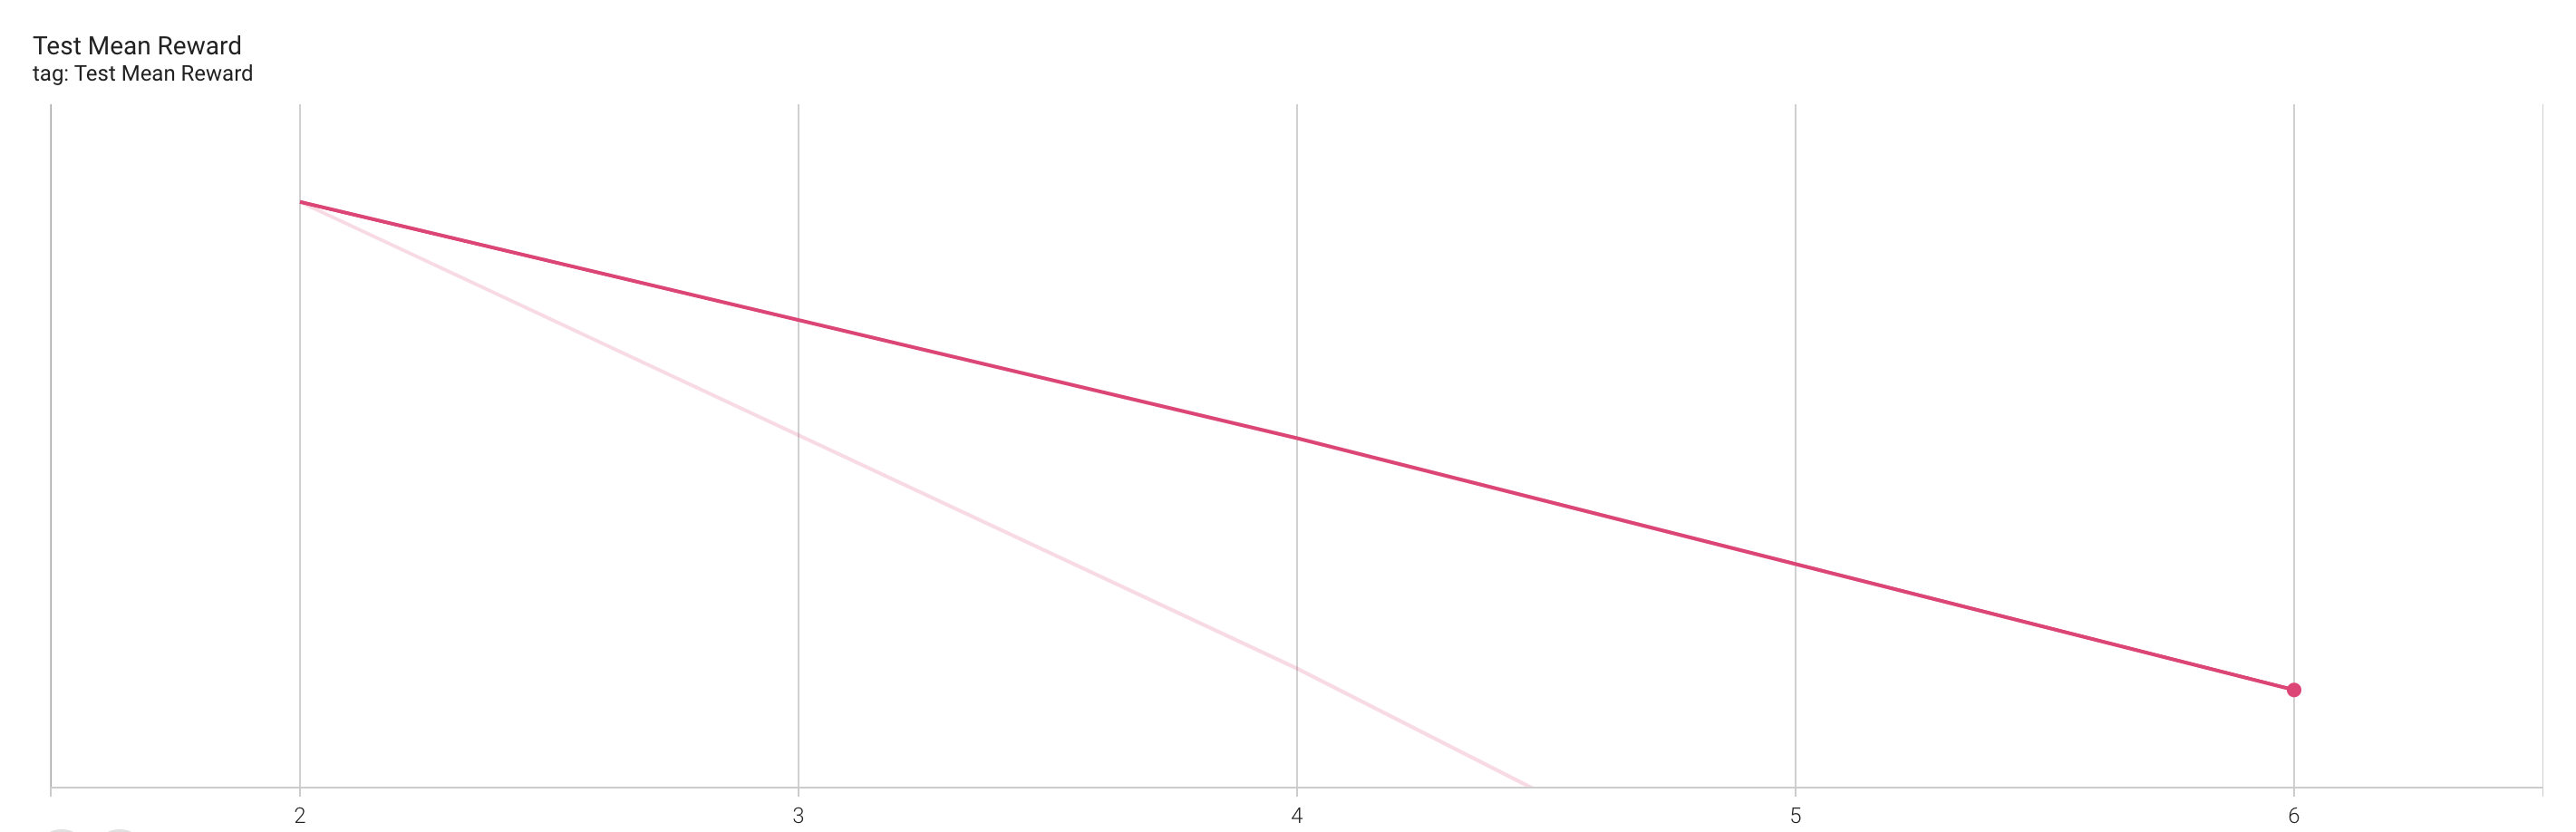
\includegraphics[width=1\textwidth]{figuras/experiments/vision transformers/test_mean_reward.png}
	\caption[Experimento \textit{Vision Transformer} - Testing reward mean]{Experimento \textit{Vision Transformer} - Testing reward mean}
	\label{fig-experimento-vision-transformer-1-testing-reward-mean}
\end{figure}
\begin{figure}[H]
	\centering
	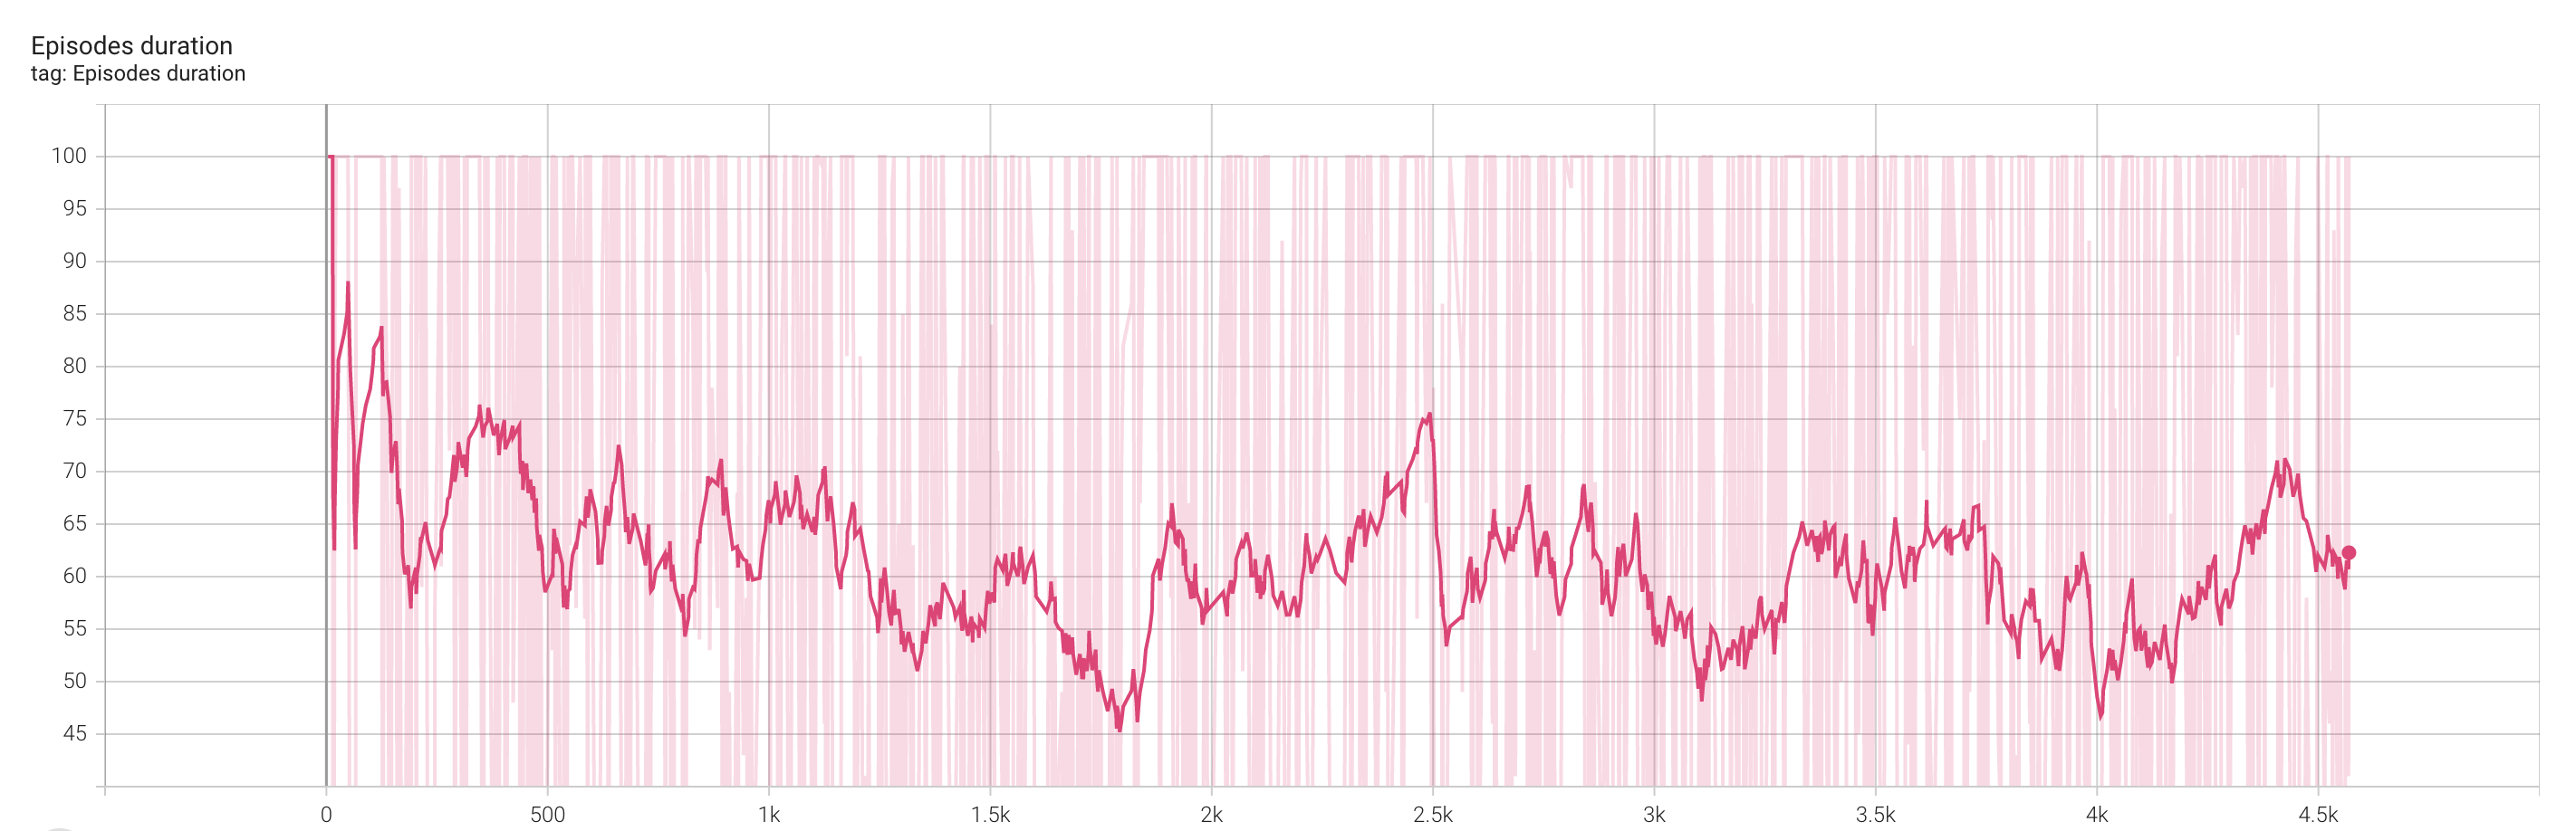
\includegraphics[width=1\textwidth]{figuras/experiments/vision transformers/episodes_duration.png}
	\caption[Experimento \textit{Vision Transformer} - Duración de los episodios]{Experimento \textit{Vision Transformer} - Duración de los episodios}
	\label{fig-experimento-vision-transformer-1-episodes-duration}
\end{figure}


\subsection{Conclusiones}
\label{resultados-conclusiones-actor-critic-experimentos}
